%% ============================================================
%% NeurIPS 2026 Submission
%% What Do Time Series Foundation Models Actually Learn?
%% A Geometric Perspective
%% ============================================================

\documentclass[10pt]{article}
\usepackage[preprint]{neurips_2026}

\usepackage{amsmath}
\usepackage{amsthm}
\usepackage{amssymb}
\usepackage{mathtools}
\usepackage{booktabs}
\usepackage{multirow}
\usepackage{graphicx}
\usepackage{xcolor}
\usepackage{microtype}
\usepackage{algorithm}
\usepackage{algpseudocode}
\usepackage[round,sort,compress]{natbib}
\usepackage{hyperref}
\usepackage{cleveref}
\usepackage[font=small,labelfont={bf},textfont={bf}]{caption}
\usepackage[section]{placeins}

\graphicspath{{figures/}}

% Tighter float/text spacing to fit 10 pages
\setlength{\textfloatsep}{8pt plus 2pt minus 3pt}
\setlength{\floatsep}{6pt plus 2pt minus 2pt}
\setlength{\intextsep}{6pt plus 2pt minus 2pt}
\setlength{\abovecaptionskip}{4pt}
\setlength{\belowcaptionskip}{2pt}

% ---- Theorem environments -------------------------------------------
\newtheorem{theorem}{Theorem}[section]
\newtheorem{proposition}[theorem]{Proposition}
\newtheorem{lemma}[theorem]{Lemma}
\newtheorem{corollary}[theorem]{Corollary}
\theoremstyle{definition}
\newtheorem{definition}[theorem]{Definition}
\newtheorem{assumption}[theorem]{Assumption}
\theoremstyle{remark}
\newtheorem{remark}[theorem]{Remark}

% ---- Math shorthands ------------------------------------------------
\newcommand{\R}{\mathbb{R}}
\newcommand{\E}{\mathbb{E}}
\newcommand{\Prob}{\mathbb{P}}
\newcommand{\Zset}{\mathcal{Z}}
\newcommand{\Mset}{\mathcal{M}}
\newcommand{\trm}{\mathcal{M}_\theta}
\newcommand{\norm}[1]{\lVert #1 \rVert}
\newcommand{\abs}[1]{\lvert #1 \rvert}
\newcommand{\inner}[2]{\langle #1,\, #2 \rangle}
\newcommand{\lcs}{\ensuremath{\mathrm{LCS}}}
\newcommand{\tsi}{\ensuremath{\mathrm{TSI}}}
\newcommand{\gsp}{\ensuremath{\mathrm{GSP}}}
\newcommand{\ltc}{\ensuremath{\mathrm{LTC}}}
\newcommand{\ltcstep}{\ensuremath{\mathrm{LTC}_{\mathrm{step}}}}
\newcommand{\ltcdir}{\ensuremath{\mathrm{LTC}_{\mathrm{dir}}}}
\newcommand{\pds}{\ensuremath{\mathrm{PDS}}}
\newcommand{\fss}{\ensuremath{\mathrm{FSS}}}
\newcommand{\css}{\ensuremath{\mathrm{CSS}}}
\newcommand{\rspear}{\ensuremath{\rho_s}}
\newcommand{\dint}{\ensuremath{d_{\mathrm{int}}}}
\newcommand{\Hb}{\ensuremath{H_b}}
\newcommand{\BalAcc}{\ensuremath{\mathrm{BalAcc}}}
\newcommand{\smax}{\ensuremath{\sigma_{\max}}}
\newcommand{\Lip}{\ensuremath{\mathrm{Lip}}}

% ---- NeurIPS checklist answer commands ------------------------------
\newcommand{\answerYes}[1]{\textbf{[Yes]} #1}
\newcommand{\answerNo}[1]{\textbf{[No]} #1}
\newcommand{\answerNA}[1]{\textbf{[N/A]} #1}

% ---- Title and authors -----------------------------------------------
\title{What Do Time Series Foundation Models Actually Learn?\\
       A Geometric Perspective}

\author{%
  Anonymous Authors\\
  Anonymous Institution\\
  \texttt{anonymous@example.com}
}

% =====================================================================
\begin{document}
\maketitle
% =====================================================================

% -----------------------------------------------------------------
\begin{abstract}
% -----------------------------------------------------------------
Time series foundation models (TSFMs) are widely deployed for zero-shot
forecasting, yet we have almost no understanding of what they actually
learn to represent---a question that forecasting accuracy alone cannot answer.
We introduce the \textbf{Latent Geometry Framework (LGF)}, a diagnostic
that characterises the representation geometry of any frozen TSFM directly
from its embeddings, requiring no retraining, labels, or gradient access.

Applied across fourteen TSFMs and six datasets, LGF surfaces three consistent
findings.
First, pretraining encodes temporal patterns selectively: seasonal and
volatility structure are linearly readable from frozen embeddings ($78.6\%$
and $70.9\%$ balanced accuracy, significantly above chance), while trend
direction is not---because window-level normalisation, applied by every
TSFM, provably removes the information needed to distinguish rising from
falling windows.
Second, training-data exposure leaves a detectable geometric fingerprint:
four models show anomalously high trajectory complexity on ETTh1---a
standard benchmark included in their pretraining corpora---that is entirely
invisible to held-out forecasting error.
Third, the local density structure of the embedding space predicts forecast
difficulty within familiar domains ($\rho = 0.41$ on Electricity) but
collapses to chance on out-of-distribution equity data ($\rho \approx 0$),
a split that holds universally across all models and provides a principled
early-warning signal for deployment outside the training distribution.
\end{abstract}

% =====================================================================
\section{Introduction}
\label{sec:intro}
% =====================================================================

Time series foundation models---TimesFM~\citep{das2024timesfm},
Chronos~\citep{ansari2024chronos}, MOMENT~\citep{goswami2024moment},
Moirai~\citep{woo2024moirai}, Time-MoE~\citep{shi2024timemoe}---pretrain
on large heterogeneous corpora and promise zero-shot transfer across energy,
climate, finance, and traffic domains.
Despite extensive benchmarking, a fundamental question remains unanswered:
\emph{what do these models actually learn to represent?}
Forecasting error cannot answer this: two TSFMs with identical test-set MAE
can encode entirely different geometric structure, with direct consequences
for when zero-shot predictions can be trusted and how models should be adapted.
\citet{zeng2023transformers} showed that a single-layer linear model matches
deep Transformer forecasters on standard benchmarks, sharpening the question
of what large-scale pretraining contributes.

For vision and language, the analogous question was resolved geometrically:
image classifiers compress onto low-dimensional manifolds with intrinsic
dimension predicting generalisation \citep{ansuini2019intrinsic};
BERT organises syntactic subspaces geometrically \citep{reif2019visualizing}.
No equivalent analysis exists for time series.

We close this gap with the \textbf{Latent Geometry Framework (LGF)}: a
four-stage diagnostic pipeline operating on frozen embeddings---no fine-tuning,
gradient access, or labels required---with a formal guarantee per metric.

\paragraph{Contributions.}
\begin{enumerate}
  \setlength{\itemsep}{2pt}\setlength{\topsep}{2pt}
  \item \textbf{Framework.} LGF measures temporal trajectory complexity (LTC),
    manifold regularity (LCS, TSI, GSP), neighbourhood reliability (PDS, FSS),
    and temporal concept encoding (CSS)---all from frozen inference alone.
  \item \textbf{Theory.} We prove a Lipschitz stability bound (TSI), a mutual
    information lower bound via Fano's inequality (CSS), conditions for PDS
    positivity, and a Wasserstein bound predicting its OOD collapse
    (Theorems~\ref{thm:tsi_main}, \ref{thm:css_main}, \ref{thm:pds_main}).
  \item \textbf{Empirics.} Every theoretical prediction is confirmed across
    four benchmarks and two OOD equity indices; LGF also differentiates ten
    additional TSFMs spanning all major pretraining paradigms
    (Table~\ref{tab:models}).
\end{enumerate}

% =====================================================================
\section{Related Work}
\label{sec:related}
% =====================================================================

\paragraph{TSFMs and the representation gap.}
The last three years have produced a rapid proliferation of TSFMs pretrained
on large heterogeneous corpora, spanning decoder-only autoregressive models
(TimesFM~\citep{das2024timesfm,das2025timesfm2}, Timer~\citep{liu2024timer}),
masked encoder-decoder architectures
(MOMENT~\citep{goswami2024moment}, Moirai~\citep{woo2024moirai},
Moirai-MoE~\citep{woo2024moiraimoe}), language-model-inspired approaches
(Chronos~\citep{ansari2024chronos}, Lag-Llama~\citep{rasul2024lagllama},
LLMTime~\citep{gruver2023llmts}), and billion-parameter sparse models
(Time-MoE~\citep{shi2024timemoe}).
Comprehensive surveys \citep{liang2024foundation,jin2023large,meyer2025tsfmreview}
and benchmarks \citep{aksu2024gifteval,qiu2024tfb,li2025tsfmbench} evaluate
these families at the output level---forecasting error on held-out splits---leaving
the structure of their learned representations entirely uncharacterised.
\citet{zeng2023transformers} sharpened this gap by showing that a single-layer
linear model matches deep Transformer forecasters on standard benchmarks:
if accuracy cannot distinguish architectures, what does large-scale pretraining
actually contribute?

\paragraph{Geometric analysis of neural representations.}
For vision and NLP, this question was resolved geometrically.
\citet{ansuini2019intrinsic} showed that intrinsic dimensionality collapses
in the final layers of image classifiers, with the collapse magnitude predicting
generalisation.
\citet{raghu2017svcca} used SVCCA to track how representations converge during
training, revealing that lower layers stabilise first.
\citet{reif2019visualizing} demonstrated that BERT organises linguistic
subspaces---syntax, coreference---as geometrically separable regions.
\citet{aghajanyan2021intrinsic} connected the intrinsic dimension of the
fine-tuning solution manifold to parameter efficiency, explaining why adapters
work.
Together these results show that geometric analysis of frozen representations
predicts generalisation, enables efficient adaptation, and exposes failure modes
that output-level evaluation misses entirely.
No analogous framework exists for time series encoders; LGF is the first.

\paragraph{Evaluation integrity and data leakage.}
A growing concern is that standard benchmarks overlap TSFM pretraining corpora.
\citet{meyer2025tsfmreview} document that Electricity and ETTh1 appear verbatim
in multiple pretraining corpora; \citet{edwards2024scalinglaws} derive scaling
laws over benchmarks that carry this leakage.
GIFT-Eval \citep{aksu2024gifteval}, TSFM-Bench \citep{li2025tsfmbench}, and
TFB \citep{qiu2024tfb} address this at the forecasting level.
LGF complements these efforts by providing a geometric signature of
memorisation---an ETTh1 $\ltcstep$ spike that is invisible to held-out
forecasting error---and uses out-of-corpus CSI300/CSI800 equity indices as a
leakage-free test for geometric transferability.

\paragraph{Explainability for time series.}
Existing XAI methods for time series
\citep{ismail2020benchmarking,theissler2022explainable} assign importance
scores to input timesteps via LIME, SHAP, or integrated gradients.
These operate at the prediction level and do not characterise what the model
has learned to represent in its latent space.
Linear probing \citep{alain2017probing} tests whether a concept is linearly
decodable from frozen representations; CSS adopts this approach but applies it
to temporal primitives---seasonality, volatility, trend---derived from STL
decomposition \citep{cleveland1990stl} without requiring external supervision.
Extended review: Appendix~\ref{app:related_full}.

% ------------------------------------------------------------------
\subsection{Preliminaries}
\label{sec:prelim}
% ------------------------------------------------------------------

\paragraph{Notation.}
Let $f_\theta: \R^L \to \R^D$ be a frozen TSFM encoder with parameters
$\theta$.
Embeddings are obtained by mean-pooling final-layer token representations
over $T{=}L/P$ patch tokens:
\[
  z_i = \frac{1}{T}\sum_{t=1}^{T} f_\theta^{(\mathcal{L})}(w_i)_t \;\in\; \R^D.
\]
We collect $N$ sliding windows $\mathcal{W}{=}\{(w_i,s_i)\}_{i=1}^N$ with
start times $s_i$, paired forecast errors $\mathcal{E}{=}\{e_i\}_{i=1}^N$,
and embeddings $\Zset{=}\{z_i\}_{i=1}^N$.
STL decomposition \citep{cleveland1990stl} of each window yields trend, seasonal,
and residual components used as concept labels in Stages~2 and~4 (no external
supervision required).

\paragraph{Temporal Representation Manifold.}
\begin{definition}[TRM]
\label{def:trm}
The \emph{Temporal Representation Manifold} is
$\trm = f_\theta(\mathrm{supp}(\mathcal{P})) \subset \R^D$,
approximated empirically by $\Zset$.
\end{definition}
\begin{assumption}[Lipschitz encoder]
\label{asm:lipschitz}
$f_\theta$ is $L_\theta$-Lipschitz.
This holds for Transformers with bounded weight norms.
\end{assumption}
Under Assumption~\ref{asm:lipschitz} and compact input support, $\trm$ is
compact and rectifiable with intrinsic dimension
$\dint \leq \min(L,D)$ (Appendix~\ref{app:manifold_proofs},
Theorems~\ref{thm:trm_rect_app}--\ref{thm:id_bound_app}).
The key consequence is that $\trm$ can be meaningfully measured: its
arc-length, cluster structure, local density, and concept-encoded directions
are all well-defined geometric quantities.

\paragraph{Geometric view of pretraining.}
We interpret pretraining as organising $\trm$ in ways that reflect temporal
structure.
A \emph{compact} manifold ($\dint \ll D$) concentrates forecast-relevant
variation; a \emph{clustered} manifold groups windows sharing temporal
primitives; a manifold with reliable \emph{local density} makes
neighbourhood isolation a proxy for forecast difficulty.
LGF formalises each of these properties with a metric and a theoretical
guarantee, operating entirely on frozen embeddings---no fine-tuning, gradient
access, or labels.

% =====================================================================
\section{Latent Geometry Framework}
\label{sec:framework}
% =====================================================================

LGF diagnoses the organisation of $\trm$ across four stages
(Figure~\ref{fig:overview_main}).
Stages~1--2 probe mapping geometry; Stage~3 links local density to forecast
quality; Stage~4 decodes temporal concept encoding.

\begin{figure}[!h]
\centering
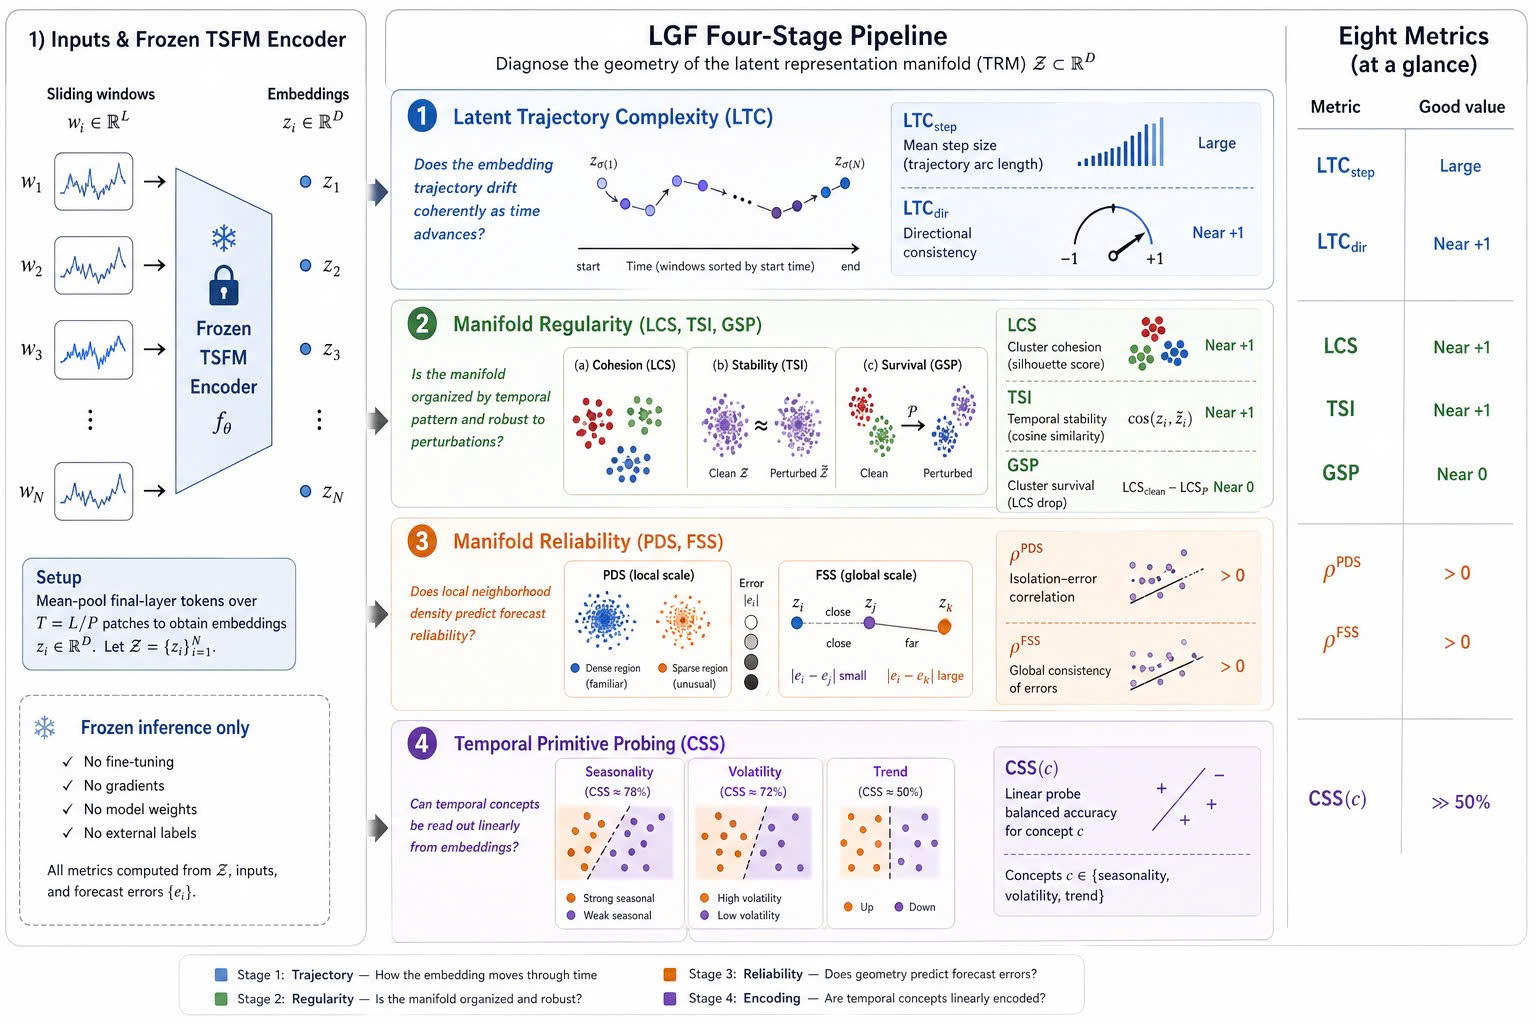
\includegraphics[width=0.88\linewidth]{overview}
\caption{LGF four-stage pipeline. \emph{Stage~1} (LTC): trajectory richness
and directional consistency. \emph{Stage~2} (Regularity): cluster structure
and perturbation stability. \emph{Stage~3} (Reliability): local neighbourhood
density vs.\ forecast error. \emph{Stage~4} (CSS): linear decodability of
temporal concepts. All stages operate on frozen embeddings only.}
\label{fig:overview_main}
\end{figure}

% ------------------------------------------------------------------
\subsection{Stage~1 --- Latent Trajectory Complexity (LTC)}
\label{sec:ltc}
% ------------------------------------------------------------------

LTC measures the \emph{richness} ($\ltcstep$: mean arc-length step) and
\emph{directionality} ($\ltcdir$: cosine consistency of consecutive steps) of
the time-ordered embedding trajectory, comparing pretrained to
randomly-initialised controls (Figure~\ref{fig:ltc_intuition},
Appendix~\ref{app:ltc_fig}).

\paragraph{Formal definition.}
Let $\sigma$ sort windows by start time $s_i$, and let
$\delta_i = z_{\sigma(i+1)} - z_{\sigma(i)}$ be the embedding step between
consecutive windows.
\begin{align}
  \ltcstep &= \frac{1}{N{-}1}\sum_{i=1}^{N-1} \norm{\delta_i}_2,
  &
  \ltcdir &= \frac{1}{N{-}2}\sum_{i=1}^{N-2}
    \frac{\delta_i \cdot \delta_{i+1}}{\norm{\delta_i}\,\norm{\delta_{i+1}}}.
  \label{eq:ltc}
\end{align}

$\ltcdir{>}0$ indicates a consistently directed trajectory; $\ltcdir{\approx}0$
a random walk.
Pretraining guarantees $\E[\ltcstep(f_\theta)] \geq \E[\ltcstep(f_{\theta_0})]$
for any random-weight control $f_{\theta_0}$
(Appendix~\ref{app:ltc_proofs}, Propositions~\ref{prop:ltc_arc}--\ref{prop:ltc_pretraining}).

% ------------------------------------------------------------------
\subsection{Stage~2 --- Manifold Regularity (LCS, TSI, GSP)}
\label{sec:regularity}
% ------------------------------------------------------------------

Regularity tests whether the embedding space is organised by temporal
structure: same-trend windows should cluster together (LCS) while remaining
stable under small perturbations (TSI, GSP).
Labels derive from input values alone via STL decomposition---no model
supervision---so positive LCS and TSI gaps reflect learned structure, not
label leakage.

\paragraph{Trend labels.}
STL decomposition \citep{cleveland1990stl} yields OLS slope $\hat{\beta}_i$
on the trend component; labels $y_i \in \{\text{up},\text{flat},\text{down}\}$
via $\hat{\beta}_i \gtrless \pm\delta\sigma_{w_i}$ ($\delta{=}0.05$).

\paragraph{Latent Cohesion Score (LCS).}
LCS is the mean silhouette score of embeddings grouped by STL trend label
(Figure~\ref{fig:lcs_clusters}, Appendix~\ref{app:reg_figs}):
\[
  \lcs = \frac{1}{N}\sum_{i=1}^N \frac{b(i) - a(i)}{\max(a(i),\,b(i))},
  \quad \lcs \in [-1,1].
\]
$\lcs{>}0$ means same-trend windows are closer to each other than to other
trends on average.
For i.i.d.\ random embeddings $\E[\lcs] \to 0$ as $D \to \infty$
(Proposition~\ref{prop:lcs_degenerate}, Appendix~\ref{app:manifold_proofs}),
so a positive LCS certifies learned structure.

\paragraph{Temporal Stability Index (TSI).}
$\tsi_{\mathcal{P}} = N^{-1}\sum_i \cos(z_i, \tilde{z}_i)$ measures cosine
similarity before/after perturbation $\mathcal{P}$: Gaussian noise ($\sigma{=}0.02$),
feature dropout ($p{=}0.05$), or time-warp ($k{=}3$).
The Lipschitz bound
$\tsi \geq (\mu - L_\theta\epsilon)/(\mu + L_\theta\epsilon)$\label{thm:tsi_main}
explains the near-unity floor for both pretrained and random encoders
(Theorem~\ref{thm:tsi_main}, Appendix~\ref{app:stability_proofs}).

\paragraph{Generalised Stability under Perturbation (GSP).}
$\gsp_{\mathcal{P}} = \lcs_{\mathrm{clean}} - \lcs_{\mathcal{P}}$ measures
the drop in cluster cohesion after perturbation; values near zero confirm that
cluster structure is robust.
A formal bound appears in Appendix~\ref{app:stability_proofs}
(Theorem~\ref{thm:gsp_bound_app}).

% ------------------------------------------------------------------
\subsection{Stage~3 --- Manifold Reliability Protocol (PDS and FSS)}
\label{sec:reliability}
% ------------------------------------------------------------------

PDS tests locally whether $k$-NN isolation predicts per-window forecast error;
FSS tests globally whether pairwise embedding distance predicts pairwise error
difference (Figure~\ref{fig:pds_concept}, Appendix~\ref{app:rel_fig}).
Formally, $\rspear^{\pds} = \mathrm{Spearman}(\bar{d}_i, |e_i|)$ where
$\bar{d}_i$ is the mean $k$-NN distance in $\Zset$ ($k{=}10$), and
$\rspear^{\fss} = \mathrm{Spearman}(\|z_i{-}z_j\|, |e_i{-}e_j|)$ over
random pairs.

\begin{theorem}[PDS Positivity and OOD Collapse]
\label{thm:pds_main}
\textbf{(i)} If error and isolation co-vary with the same distributional-shift
signal, $\rspear^{\pds} \geq 0$.
\textbf{(ii)} Under large distribution shift, all OOD embeddings land in
uniformly sparse regions of $\trm$, eliminating variance in $\bar{d}_i$, so
$\rspear^{\pds} \to 0$.
\textbf{(iii)} There exist configurations where $\rspear^{\pds} \gg \rspear^{\fss}$;
global distances cannot recover the local density signal.
\emph{(Proof: Appendix~\ref{app:reliability_proofs}.)}
\end{theorem}

Theorem~\ref{thm:pds_main}(ii) makes a sharp prediction: PDS collapses on OOD
data while encoder-level properties (LTC, CSS) remain.
Section~\ref{sec:results} tests this directly.

% ------------------------------------------------------------------
\subsection{Stage~4 --- Temporal Primitive Probing (CSS)}
\label{sec:css}
% ------------------------------------------------------------------

CSS measures which temporal primitives---trend direction, seasonality,
volatility---are linearly decodable from frozen embeddings.
$\css{>}50\%$ means the concept occupies geometrically separable regions of
$\R^D$; the margin above chance lower-bounds the mutual information the
embedding carries about that concept.

\paragraph{Class Separation Score (CSS).}
Labels derive from STL decomposition of input values only:
seasonality = above/below-median seasonal-component strength;
volatility = above/below-median residual variance;
trend = above/below-median trend slope.
CSS is the balanced accuracy of an $\ell_2$-regularised logistic probe
($C{=}1$) on a held-out 20\% stratified split:
\begin{equation}
  \css(c) = \BalAcc\!\left(\hat{\mathbf{y}}^c,\, \mathbf{y}^c\right),
  \quad c \in \{\mathrm{trend},\,\mathrm{season},\,\mathrm{vol}\}.
  \label{eq:css}
\end{equation}

\begin{theorem}[CSS and Mutual Information]
\label{thm:css_main}
\textbf{(i)} $\css(c) > 1/2$ iff Fisher discriminant ratio $J_F > 0$
(concept occupies geometrically distinct regions).
\textbf{(ii)} $\css(c) = \alpha$ implies $I(Z;\,Y^c) \geq 1 - \Hb(1{-}\alpha)$
bits of mutual information.
\textbf{(iii)} The pretrained--random CSS gap lower-bounds the information
gained from pretraining by $\Hb(1{-}\alpha_r) - \Hb(1{-}\alpha_p)$ bits.
\emph{(Proof: Appendix~\ref{app:probing_proofs}.)}
\end{theorem}

\paragraph{Trend CSS and window normalisation.}
Window-level mean--variance normalisation collapses the class centroids for
trend direction ($J_F \approx 0$), driving trend CSS to near chance regardless
of pretraining quality.
This is a structural consequence of normalisation, not a model failure, and
applies to any window-normalised TSFM.
Significance is assessed via permutation test
($n_{\mathrm{perm}}{=}60$ for main benchmarks; $20$ for OOD analyses).

\paragraph{Algorithm summary.}
The full four-stage pipeline is summarised in Algorithm~\ref{alg:lgf}.

\begin{algorithm}[t]
\caption{LGF Analysis Pipeline}
\label{alg:lgf}
\begin{algorithmic}
\Require Frozen TSFM $f_\theta$;
         windows $\mathcal{W}{=}\{(w_i, s_i)\}_{i=1}^N$;
         forecast errors $\mathcal{E}{=}\{e_i\}_{i=1}^N$
\Ensure  $\ltcstep, \ltcdir$;\ $\lcs, \tsi, \gsp$;\
         $\rspear^{\pds}, \rspear^{\fss}$;\ $\css^c$
\State Extract final-layer embeddings $\Zset{=}\{z_i\}$ via mean-pooling
       \Comment{frozen inference only}
\State Sort by start time $s_i$; compute $\ltcstep, \ltcdir$
       (Eq.~\ref{eq:ltc}) \Comment{Stage 1: trajectory}
\State Derive STL trend labels $\mathbf{y}$ (\S\ref{sec:regularity});
       compute $\lcs$
\For{each perturbation type $\mathcal{P}$}
  \State Compute $\tsi_{\mathcal{P}}$ and
         $\gsp_{\mathcal{P}} = \lcs_{\mathrm{clean}} - \lcs_{\mathcal{P}}$
         \Comment{Stage 2: regularity}
\EndFor
\State Build $k$-NN graph ($k{=}10$); compute $\rspear^{\pds}$ and
       $\rspear^{\fss}$ (\S\ref{sec:reliability})
       \Comment{Stage 3: reliability}
\For{each concept $c \in \{\mathrm{trend},\mathrm{season},\mathrm{vol}\}$}
  \State Derive STL labels; train $\ell_2$ logistic probe;
         compute $\css(c)$ (Eq.~\ref{eq:css})
         \Comment{Stage 4: encoding}
\EndFor
\end{algorithmic}
\end{algorithm}

% =====================================================================
\section{Experiments}
\label{sec:experiments}
% =====================================================================

\subsection{Setup}
\label{sec:setup_exp}

\paragraph{Models.}
\noindent
\begin{minipage}[t]{0.49\textwidth}
\vspace{0pt}
We report full LGF results for \textbf{TimesFM~2.0}
\citep{das2024timesfm,das2025timesfm2}, a 500M-parameter decoder-only
Transformer pretrained on next-patch prediction ($D{=}1{,}024$).
Three supervised baselines are trained per-dataset: a two-layer \textbf{LSTM}
(hidden 128), a three-block \textbf{TCN} (channels 128, kernel 3), and a
three-layer \textbf{Transformer} ($d{=}128$, 8 heads), all with AdamW
($\mathrm{lr}{=}3{\times}10^{-4}$) and walk-forward cross-validation.
LGF results for \textbf{Chronos-Small} \citep{ansari2024chronos} (46M),
\textbf{MOMENT-Large} \citep{goswami2024moment} (385M), and \textbf{Moirai}
\citep{woo2024moirai} (311M) appear alongside TimesFM~2.0 in all tables.
\end{minipage}%
\hfill
\begin{minipage}[t]{0.47\textwidth}
\vspace{0pt}
\centering
\captionof{table}{\textbf{TSFMs evaluated.} $D$: embed.\ dim.}
\label{tab:models}
\small\setlength{\tabcolsep}{2pt}
\begin{tabular}{llrl}
\toprule
\textbf{Model} & \textbf{Family} & \textbf{Params} & \textbf{$D$}\\
\midrule
TimesFM~2.0   & Dec.-only AR    & 500M & 1024\\
Chronos-Small & Enc.-dec.\ (q.) &  46M &  512\\
MOMENT-Large  & Masked enc.     & 385M & 1024\\
Moirai        & M.\ enc.-dec.   & 311M &  768\\
\bottomrule
\end{tabular}
\end{minipage}

\paragraph{Datasets.}
Four standard long-horizon benchmarks (Electricity, ETTh1, Weather, Traffic)
plus two Chinese equity indices (CSI300, CSI800) as out-of-distribution (OOD)
validation (Table~\ref{tab:datasets}, Appendix~\ref{app:exp_details}).
The equity indices lie outside any known TSFM pretraining corpus.

\paragraph{Extraction protocol.}
$N{=}3{,}000$ sliding windows per dataset (length $L{=}512$, stride 64),
each normalised by window-level mean and standard deviation.
Forecast errors at horizons $H \in \{96, 192, 336, 720\}$.
All metrics: median with 95\% bootstrap CI (1{,}000 resamples).

\paragraph{Random-weight control.}
All TimesFM measurements are repeated on a randomly-initialised TimesFM
(same architecture, no pretrained weights).
A significant gap ($p{<}0.05$, Wilcoxon signed-rank across four datasets)
is the criterion for attributing structure to pretraining.

\subsection{Main Results}
\label{sec:results}

We first characterised how pretraining shapes the latent trajectory of frozen
embeddings.
Measuring $\ltcstep$ and $\ltcdir$ on TimesFM~2.0 across all four benchmarks,
we found that pretrained embeddings consistently produce richer, more directed
trajectories than those of a randomly-initialised encoder of identical
architecture ($\Delta{=}0.74$--$1.58$, $p{<}0.05$ Wilcoxon across datasets,
Table~\ref{tab:ltc}), confirming Proposition~\ref{prop:ltc_pretraining}.
At the same time, TimesFM sits $3.5\times$ below the per-dataset Transformer
($\ltcstep{=}4.64$ vs.\ $16.16$ on Electricity), which occupies the
memorisation regime.
This positions the pretrained encoder in a compact, structured zone between
random scatter and dataset-specific over-fitting---consistent with the
generalisation bound in Theorem~\ref{thm:gen_bound_app}
(Figure~\ref{fig:ltc_profile}).
Figure~\ref{fig:umap_pretrained_vs_random} shows the UMAP projections for
both models.
The clouds look broadly similar at this scale---UMAP discards magnitude
information---but the trajectory statistics differ quantitatively:
$\ltcstep{=}4.64$ vs.\ $3.90$ ($+19\%$, $p{<}0.05$), and the start/end
anchors of the temporal path are visibly closer together in the pretrained
model, reflecting higher directional consistency.

\begin{figure}[t]
\centering
\begin{minipage}[b]{0.46\linewidth}
  \centering
  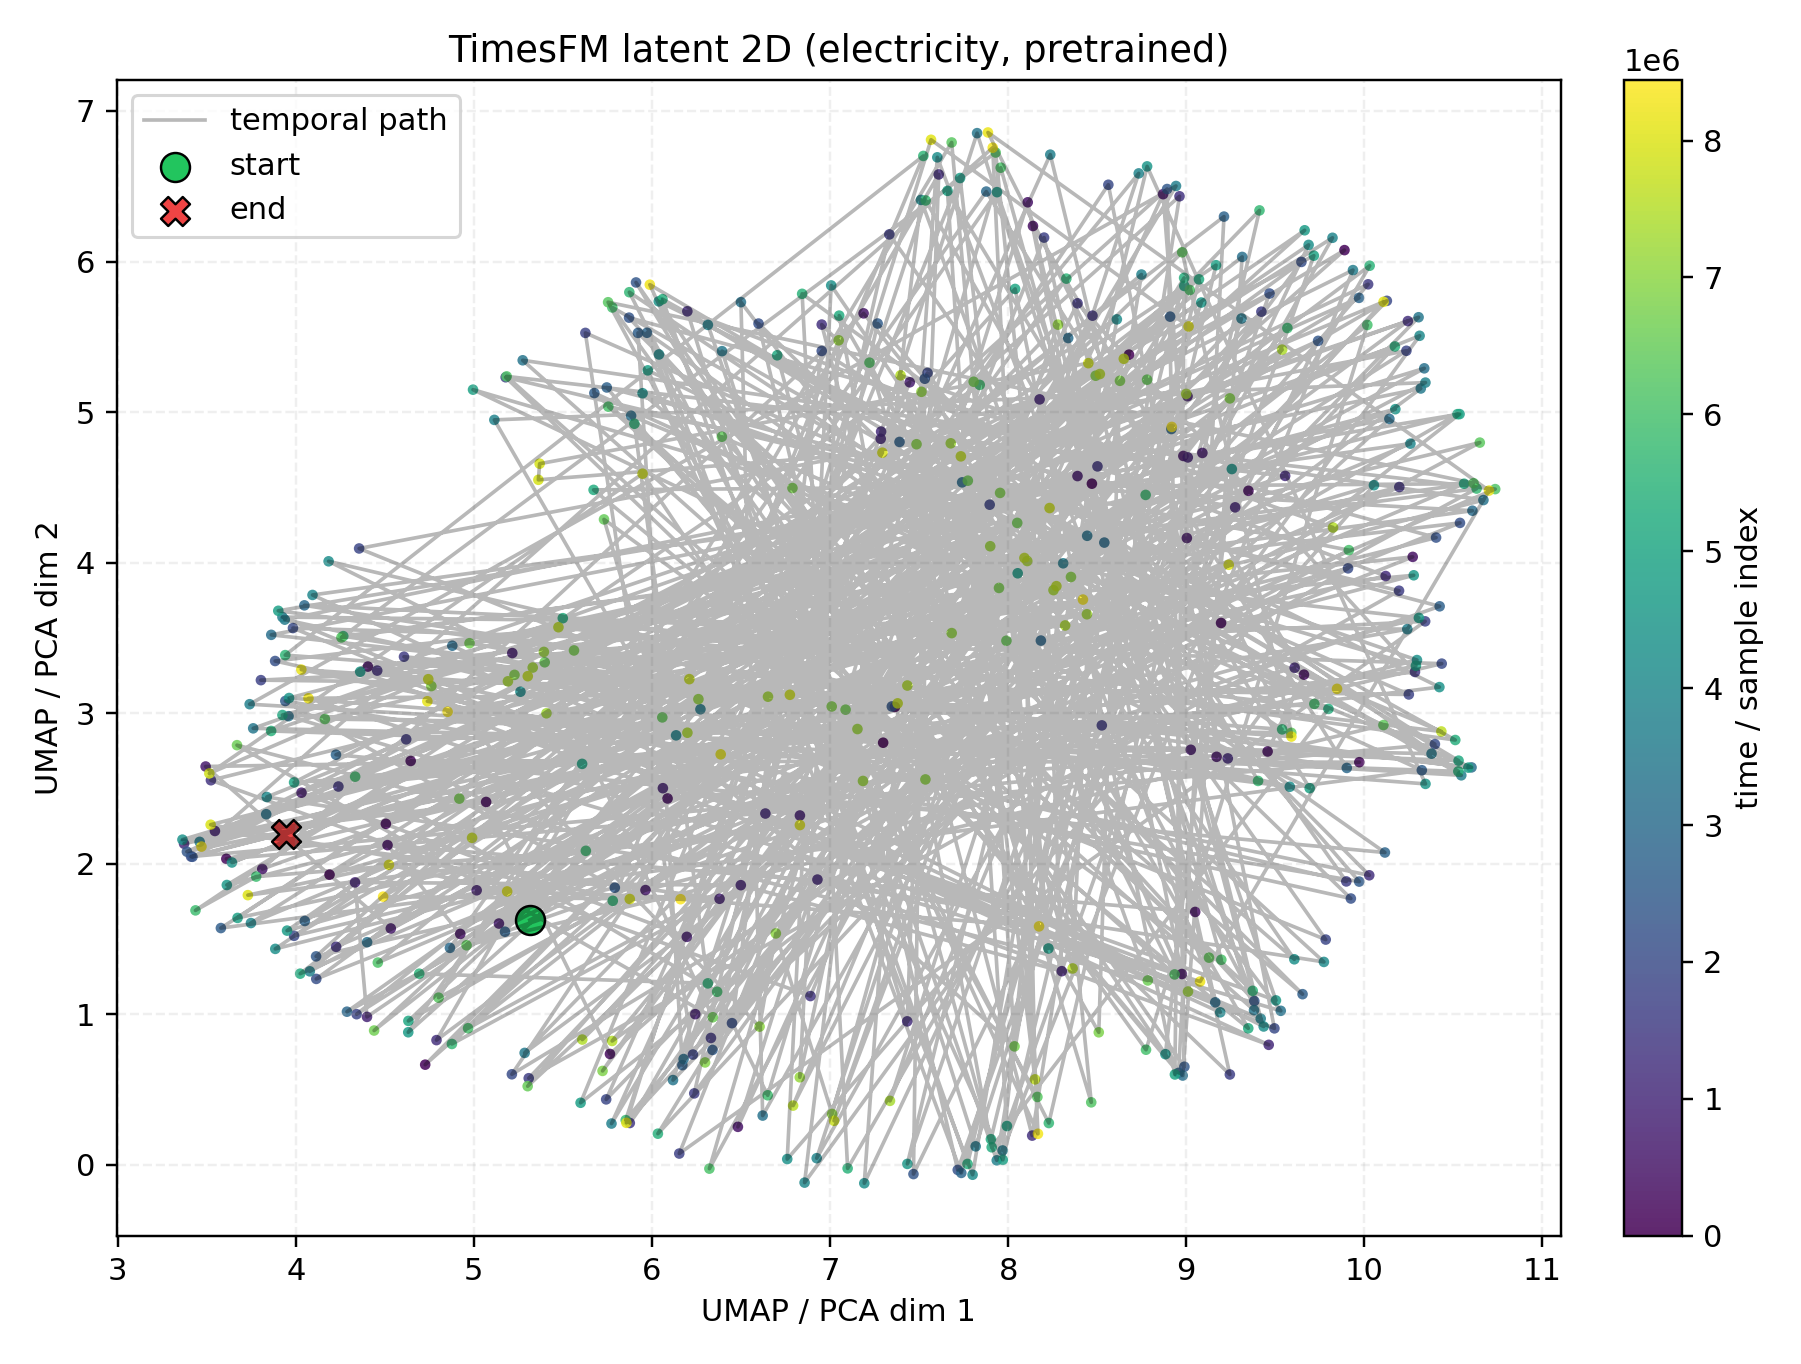
\includegraphics[width=\linewidth]{fig_umap_elec_pretrained}\\[2pt]
  \small\textbf{(a) Pretrained TimesFM}
\end{minipage}
\hfill
\begin{minipage}[b]{0.46\linewidth}
  \centering
  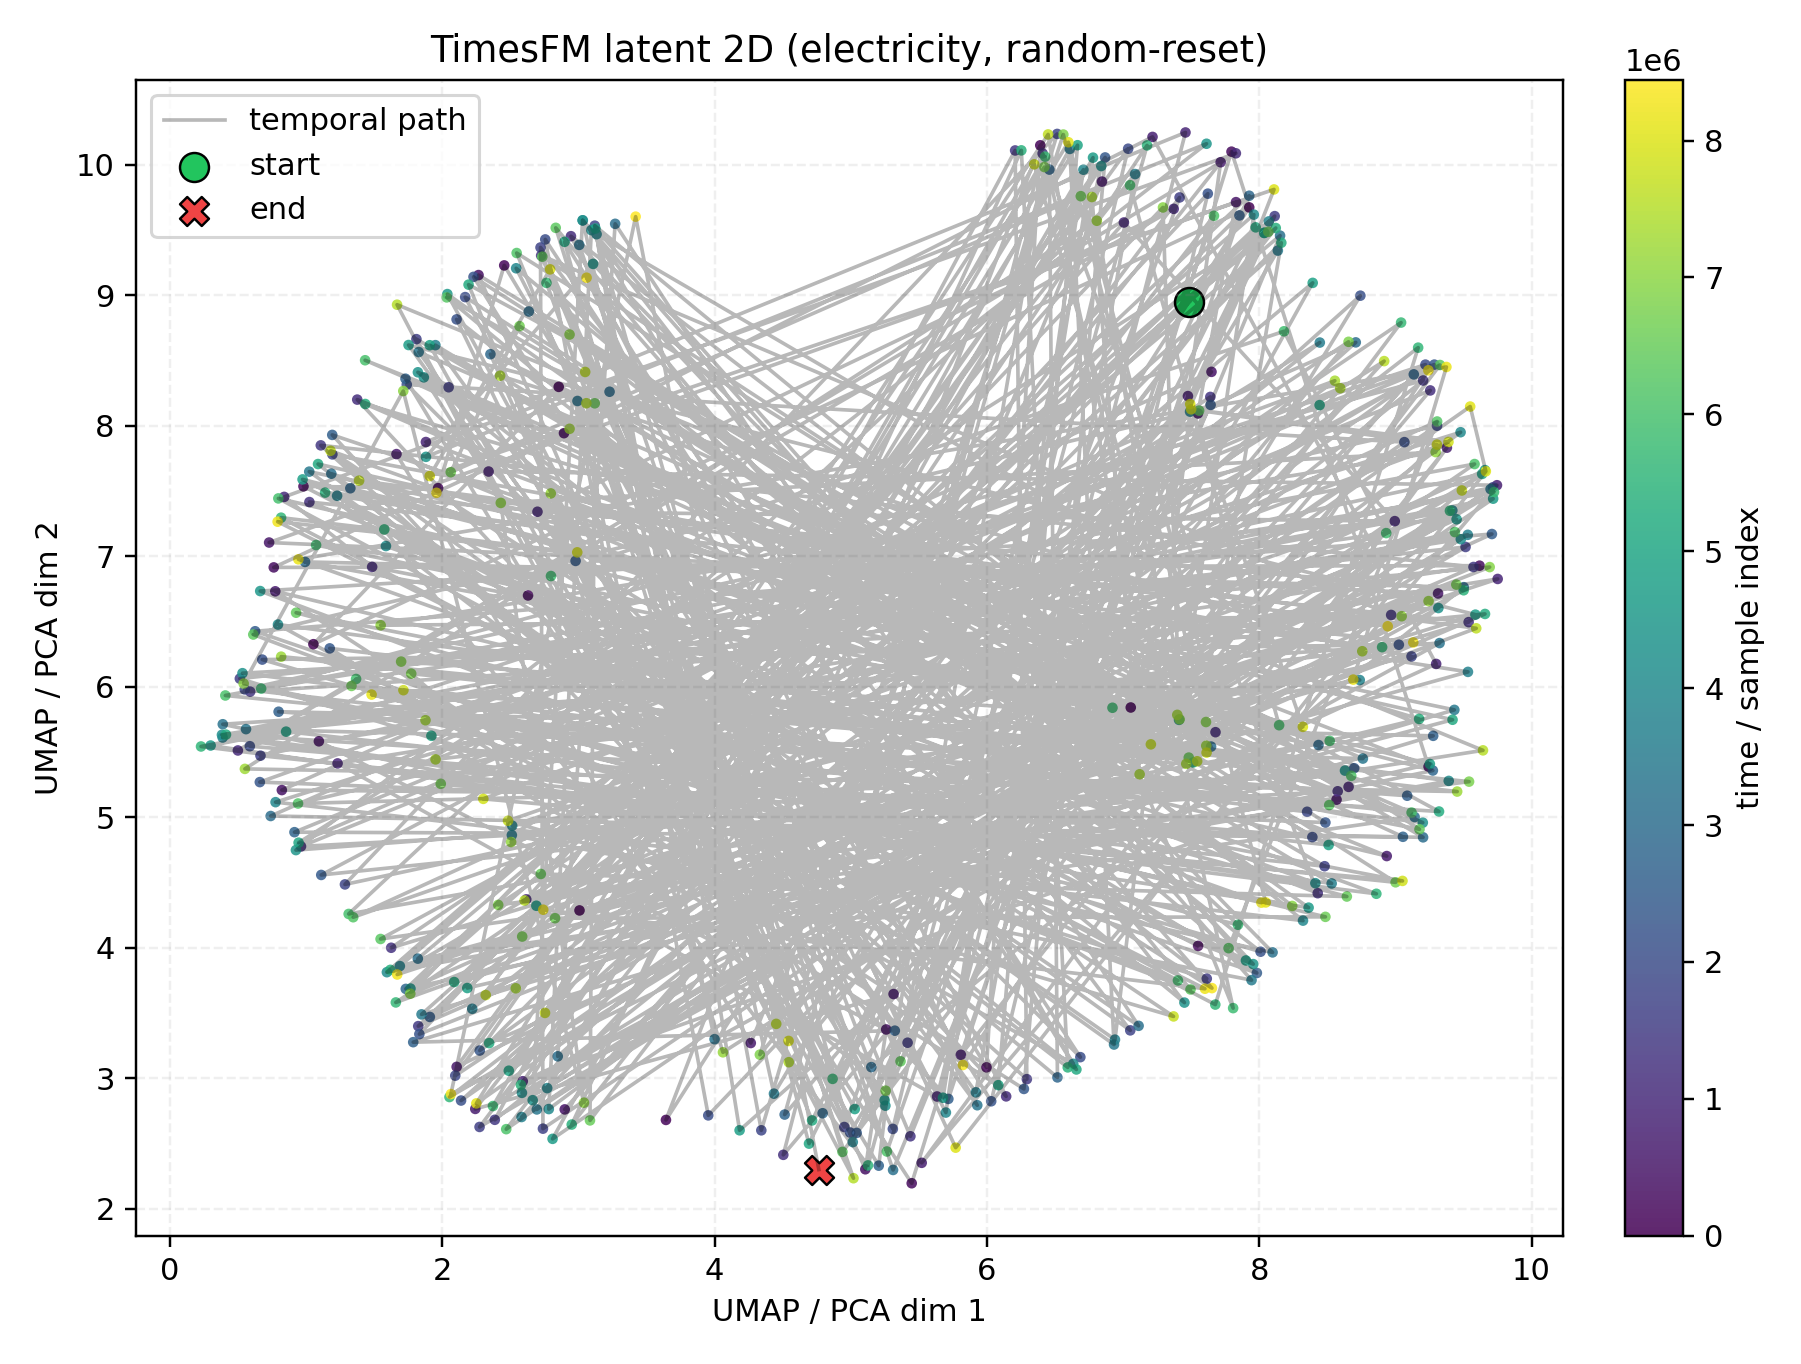
\includegraphics[width=\linewidth]{fig_umap_elec_random}\\[2pt]
  \small\textbf{(b) Random-weight control}
\end{minipage}
\caption{\textbf{UMAP projections of frozen TimesFM~2.0 embeddings on
  Electricity (3{,}000 windows, coloured by temporal index).}
  Grey lines trace the time-ordered path; green circle = start, red X = end.
  The two clouds look broadly similar at this scale, which is expected:
  UMAP discards magnitude information and both models operate in the same
  1{,}024-D space.
  The quantitative difference is in the trajectory statistics:
  $\ltcstep = 4.64$ (pretrained, a) vs.\ $3.90$ (random, b),
  a $+19\%$ gap significant at $p{<}0.05$ (Wilcoxon).
  Visually, the start and end anchors are notably closer in (a) than in (b),
  consistent with the higher directional consistency ($\ltcdir$) of the
  pretrained trajectory.}
\label{fig:umap_pretrained_vs_random}
\end{figure}

\begin{figure}[t]
\centering

\includegraphics[width=0.92\linewidth]{fig_ltc_profile}
\caption{\textbf{LTC step ($\ltcstep$) across datasets and model types.}
  \emph{Left}: pretrained TimesFM consistently exceeds the random-weight
  control across all four benchmarks.
  \emph{Right}: on Electricity, TimesFM ($4.64$) sits $3.5\times$ below
  the supervised Transformer ($16.16$) yet $19\%$ above the random encoder
  ($3.90$)---the compact structured zone between scatter and memorisation.}
\label{fig:ltc_profile}
\end{figure}

Examining the full set of fourteen TSFMs revealed two particularly informative
diagnostic patterns (Table~\ref{tab:ltc}).
Notably, four models---OFA ($\ltcstep{=}17.69$), UniTime ($28.90$),
TiRex ($25.53$), and Moirai ($26.66$)---exhibited a sharp spike on ETTh1
that did not appear on any other benchmark, with values exceeding the
supervised Transformer.
This ETTh1-specific signature is consistent with verbatim inclusion of ETTh1
in these models' pretraining corpora, and is invisible to held-out forecasting
metrics.
At the opposite extreme, Chronos-Small's value quantisation compressed
trajectory richness to $\ltcstep{=}0.13$ on Electricity---a $124\times$
reduction relative to the supervised Transformer---an encoding artefact
detectable from frozen embeddings alone.

We next asked whether local embedding density carries a signal about
per-window forecast quality, a question formalised by PDS.
On Electricity we found a strong and significant correlation between
neighbourhood isolation and forecast error ($\rspear^{\pds}{=}0.41$,
$p{<}10^{-20}$), with a positive signal also on Traffic
($\rspear^{\pds}{=}0.25$, $p{<}0.001$, Table~\ref{tab:geodesic}).
The gap over the global pairwise metric FSS reached $\Delta\rho{=}0.40$ and
$0.20$ on these two datasets, confirming that local density carries
information that pairwise distances cannot recover
(Theorem~\ref{thm:pds_main}(iii)).
The randomly-initialised encoder reversed the sign on Electricity to
$\rho{=}{-}0.34$, establishing that the reliability signal requires learned
geometry, not merely architecture.
Across ten additional TSFMs, PDS was absent or negative for eight models,
while FSS was uniformly negative for all ten ($-0.24$ to $-0.95$),
confirming that global pairwise distance is a universal negative control for
this task.
Figure~\ref{fig:geodesic} visualises this contrast per dataset: the dark blue
PDS bars exceed the light blue FSS bars on Electricity and Traffic by a
substantial margin, while the random-weight control (red) consistently sits
near zero or below, providing a direct visual confirmation of
Theorem~\ref{thm:pds_main}(iii).

\begin{figure}[t]
\centering

\includegraphics[width=0.92\linewidth]{fig_geodesic_reliability}
\caption{\textbf{PDS vs.\ FSS Spearman correlation per dataset at $H{=}96$.}
  \textbf{Dark blue}: pretrained PDS (local neighbourhood density).
  \textbf{Light blue}: pretrained FSS (global pairwise distance).
  \textbf{Red/pink}: random-weight control.
  PDS substantially exceeds FSS on Electricity ($\Delta\rho{=}0.40$) and
  Traffic ($\Delta\rho{=}0.20$); the random-weight control shows no positive
  signal, confirming that local density is learned, not architectural.
  Error bars are 95\% bootstrap CIs.}
\label{fig:geodesic}
\end{figure}

\begin{table}[t]
\begin{minipage}[t]{0.53\linewidth}
\centering
\captionof{table}{\textbf{$\ltcstep$ (higher = richer trajectory).}
\textbf{Bold} ETTh1 $>15$: memorisation spike.
Full 14-model results: Table~\ref{tab:ltc_ext} (App.~\ref{app:ablations}).}
\label{tab:ltc}
\small\setlength{\tabcolsep}{3pt}
\begin{tabular}{lccccc}
\toprule
\textbf{Model} & \textbf{Elec.} & \textbf{Wea.} & \textbf{ETTh1} & \textbf{Traf.} & $\Delta$\\
\midrule
TimesFM (pre) & 4.64 & 5.10 & 5.02 & 3.77 & $+$1.21\\
TimesFM (rnd) & 3.90 & 3.52 & 3.70 & 2.55 & ---\\
$\Delta$      & $+$0.74 & $+$1.58 & $+$1.32 & $+$1.22 & \\
\midrule
LSTM   & 4.75  & --- & --- & --- & ---\\
TCN    & 5.56  & --- & --- & --- & ---\\
Trans. & 16.16 & --- & --- & --- & ---\\
\midrule
\multicolumn{6}{l}{\textit{ETTh1 spikes \& Chronos:}}\\
OFA     & 1.00 & 1.68 & \textbf{17.69} & 1.62 & ---\\
UniTime & 3.30 & 2.68 & \textbf{28.90} & 3.86 & ---\\
TiRex   & 9.62 & 2.82 & \textbf{25.53} & 8.89 & ---\\
Moirai  & 9.97 & 2.91 & \textbf{26.66} & 9.64 & ---\\
Chronos-S & 0.13 & 0.19 & 0.21 & 0.15 & ---\\
\bottomrule
\end{tabular}
\end{minipage}%
\hfill
\begin{minipage}[t]{0.44\linewidth}
\centering
\captionof{table}{\textbf{PDS vs.\ FSS ($\rspear$) at $H{=}96$.}
$^\dagger$$p{>}0.05$.
Full 10-TSFM OOD results: Table~\ref{tab:geodesic_ext} (App.~\ref{app:ablations}).}
\label{tab:geodesic}
\small\setlength{\tabcolsep}{3pt}
\begin{tabular}{lcccc}
\toprule
& \multicolumn{2}{c}{\textbf{Pretrained}}
& \multicolumn{2}{c}{\textbf{Random}}\\
\cmidrule(r){2-3}\cmidrule(l){4-5}
\textbf{Dataset} & $\rho^{\pds}$ & $\rho^{\fss}$ & $\rho^{\pds}$ & $\rho^{\fss}$\\
\midrule
\multicolumn{5}{l}{\textit{TimesFM 2.0}}\\
Electricity & $\mathbf{0.41}$ & $0.01$  & $-0.34$ & $0.13$\\
ETTh1       & $0.04$          & $-0.01$ & $-0.27$ & $-0.01$\\
Weather     & $0.11$          & $0.09$  & $0.10$  & $0.10$\\
Traffic     & $\mathbf{0.25}$ & $0.05$  & $0.08$  & $0.12$\\
\cmidrule(r){2-3}\cmidrule(l){4-5}
Mean        & $\mathbf{0.20}$ & $0.04$  & $-0.11$ & $0.09$\\
\midrule
\multicolumn{5}{l}{\textit{OOD equity}}\\
CSI300 & $0.02^\dagger$ & $-0.07^\dagger$ & $-0.37$ & $0.07$\\
CSI800 & $-0.09^\dagger$& $-0.08^\dagger$ & $-0.38$ & $0.02^\dagger$\\
\bottomrule
\end{tabular}
\end{minipage}
\end{table}

To characterise which temporal concepts are explicitly encoded in the embedding
geometry, we trained $\ell_2$-regularised linear probes on STL-derived labels
for trend, seasonality, and volatility.

\noindent
\begin{minipage}[t]{0.42\textwidth}
\vspace{0pt}
We found that seasonality and volatility are consistently and significantly
decodable from frozen TimesFM embeddings across all four datasets
($\css{=}78.6\%$ and $70.9\%$, $p{<}0.05$), outperforming the random-weight
control by $+10.1$ and $+7.8$~pp (Table~\ref{tab:probing};
per-dataset: Table~\ref{tab:probing_detail}, App.~\ref{app:probing_detail}).
By Theorem~\ref{thm:css_main}(ii), these gaps imply at least $0.33$~bits of
mutual information about seasonality and $0.13$~bits about volatility.
Trend CSS was weak and inconsistent: a structural consequence of window-level
normalisation removing the global offset needed to separate trend directions,
as Theorem~\ref{thm:css_main}(i) predicts.
\end{minipage}%
\hfill
\begin{minipage}[t]{0.55\textwidth}
\vspace{0pt}
\centering
\captionof{table}{\textbf{CSS balanced accuracy (\%) over four datasets.}
\textbf{Bold}: $p{<}0.05$. $^\dagger$: not sig. Chance ${\approx}50\%$.}
\label{tab:probing}
\small\setlength{\tabcolsep}{2pt}
\begin{tabular}{lcccccc}
\toprule
& \multicolumn{3}{c}{\textbf{4-dataset avg.}}
& \multicolumn{3}{c}{\textbf{OOD equity}}\\
\cmidrule(r){2-4}\cmidrule(l){5-7}
\textbf{Model} & \textbf{Tr.} & \textbf{Sea.} & \textbf{Vol.}
  & \textbf{Tr.} & \textbf{Sea.} & \textbf{Vol.}\\
\midrule
TimesFM (Pre) & $67.9^\dagger$ & \textbf{78.6} & \textbf{70.9}
              & $56.9^\dagger$ & \textbf{70.0} & \textbf{65.0}\\
TimesFM (Rnd) & 63.6 & 68.5 & 63.1 & 57.3 & 55.8 & 48.1\\
\midrule
$\Delta$ & $+4.3$ & $\mathbf{+10.1}$ & $\mathbf{+7.8}$ & $-0.5$ & $\mathbf{+14.1}$ & $\mathbf{+17.0}$\\
\bottomrule
\end{tabular}
\end{minipage}

\begin{figure}[!t]
\centering

\includegraphics[width=0.74\linewidth]{fig_probing_heatmap}
\caption{\textbf{Temporal primitive probing: balanced accuracy (\%)} of a linear
classifier on frozen TimesFM~2.0 embeddings.
Pretrained (\emph{left}) consistently outperforms random-weight control
(\emph{right}) for seasonality and volatility across all four datasets.}
\label{fig:probing}
\end{figure}
\FloatBarrier

The most stringent test of LGF's predictions was the out-of-distribution
evaluation on Chinese equity indices (CSI300 and CSI800), which are absent from
all known TSFM pretraining corpora.
Theorem~\ref{thm:pds_main}(ii) predicts a three-way split: encoder-level
properties (LTC, CSS) should transfer while neighbourhood reliability (PDS)
should collapse.
This is precisely what we observed.
Pretrained $\ltcstep$ exceeded the random control on CSI300 ($4.24$
vs.\ $3.80$), and seasonality CSS reached $74.8\%$ and $70.0\%$ on the two
indices ($p{<}0.05$, up to $+18$~pp over random).
Neighbourhood reliability, however, collapsed completely: PDS fell to $0.02$
and $-0.09$ (both $p{>}0.3$, Table~\ref{tab:geodesic}).
To verify that this three-way split generalises beyond TimesFM, we evaluated
all ten additional TSFMs on the same OOD indices.
Across every model, $\rspear^{\pds}$ ranged from $-0.01$ to $-0.29$, with no
model showing a positive reliability signal---universally confirming
Theorem~\ref{thm:pds_main}(ii).
Figure~\ref{fig:ood_summary} presents the full three-way split in a single
view: the top row shows that pretrained LTC exceeds the random baseline on
both equity indices (transfer); the middle row shows CSS seasonality above
chance (transfer); the bottom row shows PDS collapsing to near-zero across
both OOD datasets (collapse).
Figure~\ref{fig:pds_density_comparison} shows the mechanism: the mean
$k$-NN distance $\bar{d}_i$ spans approximately $2$--$7$ on Electricity
(range $\approx{5}$), creating the isolation contrast that yields
$\rspear^{\pds}{=}0.41$; on CSI300 the range compresses to
${\approx}2.25$--$4.0$ (range $\approx{1.75}$), removing the variance in
$\bar{d}_i$ that PDS requires, and driving $\rspear^{\pds}$ to $0.02$.
Additional embedding geometry visualisations appear in
Appendix~\ref{app:stock_ood}; ablation results in Appendix~\ref{app:ablations}.

\begin{figure}[!ht]
\centering

\includegraphics[width=0.82\linewidth]{fig_ood_summary}
\caption{\textbf{OOD validation: LTC and CSS transfer; PDS collapses.}
  Each panel compares pretrained (blue) vs.\ random-weight (red) TimesFM.
  \emph{Top row}: $\ltcstep$ --- pretrained exceeds random on all datasets,
  including OOD equity (right column, red border), confirming trajectory
  structure transfers.
  \emph{Middle row}: CSS seasonality (\%) --- pretrained remains above chance
  and above random in both in-distribution and OOD settings.
  \emph{Bottom row}: PDS $\rspear$ --- positive within distribution;
  collapses to near-zero on OOD equity, exactly as Theorem~\ref{thm:pds_main}(ii) predicts.}
\label{fig:ood_summary}
\end{figure}

\begin{figure}[!ht]
\centering
\begin{minipage}[b]{0.43\linewidth}
  \centering
  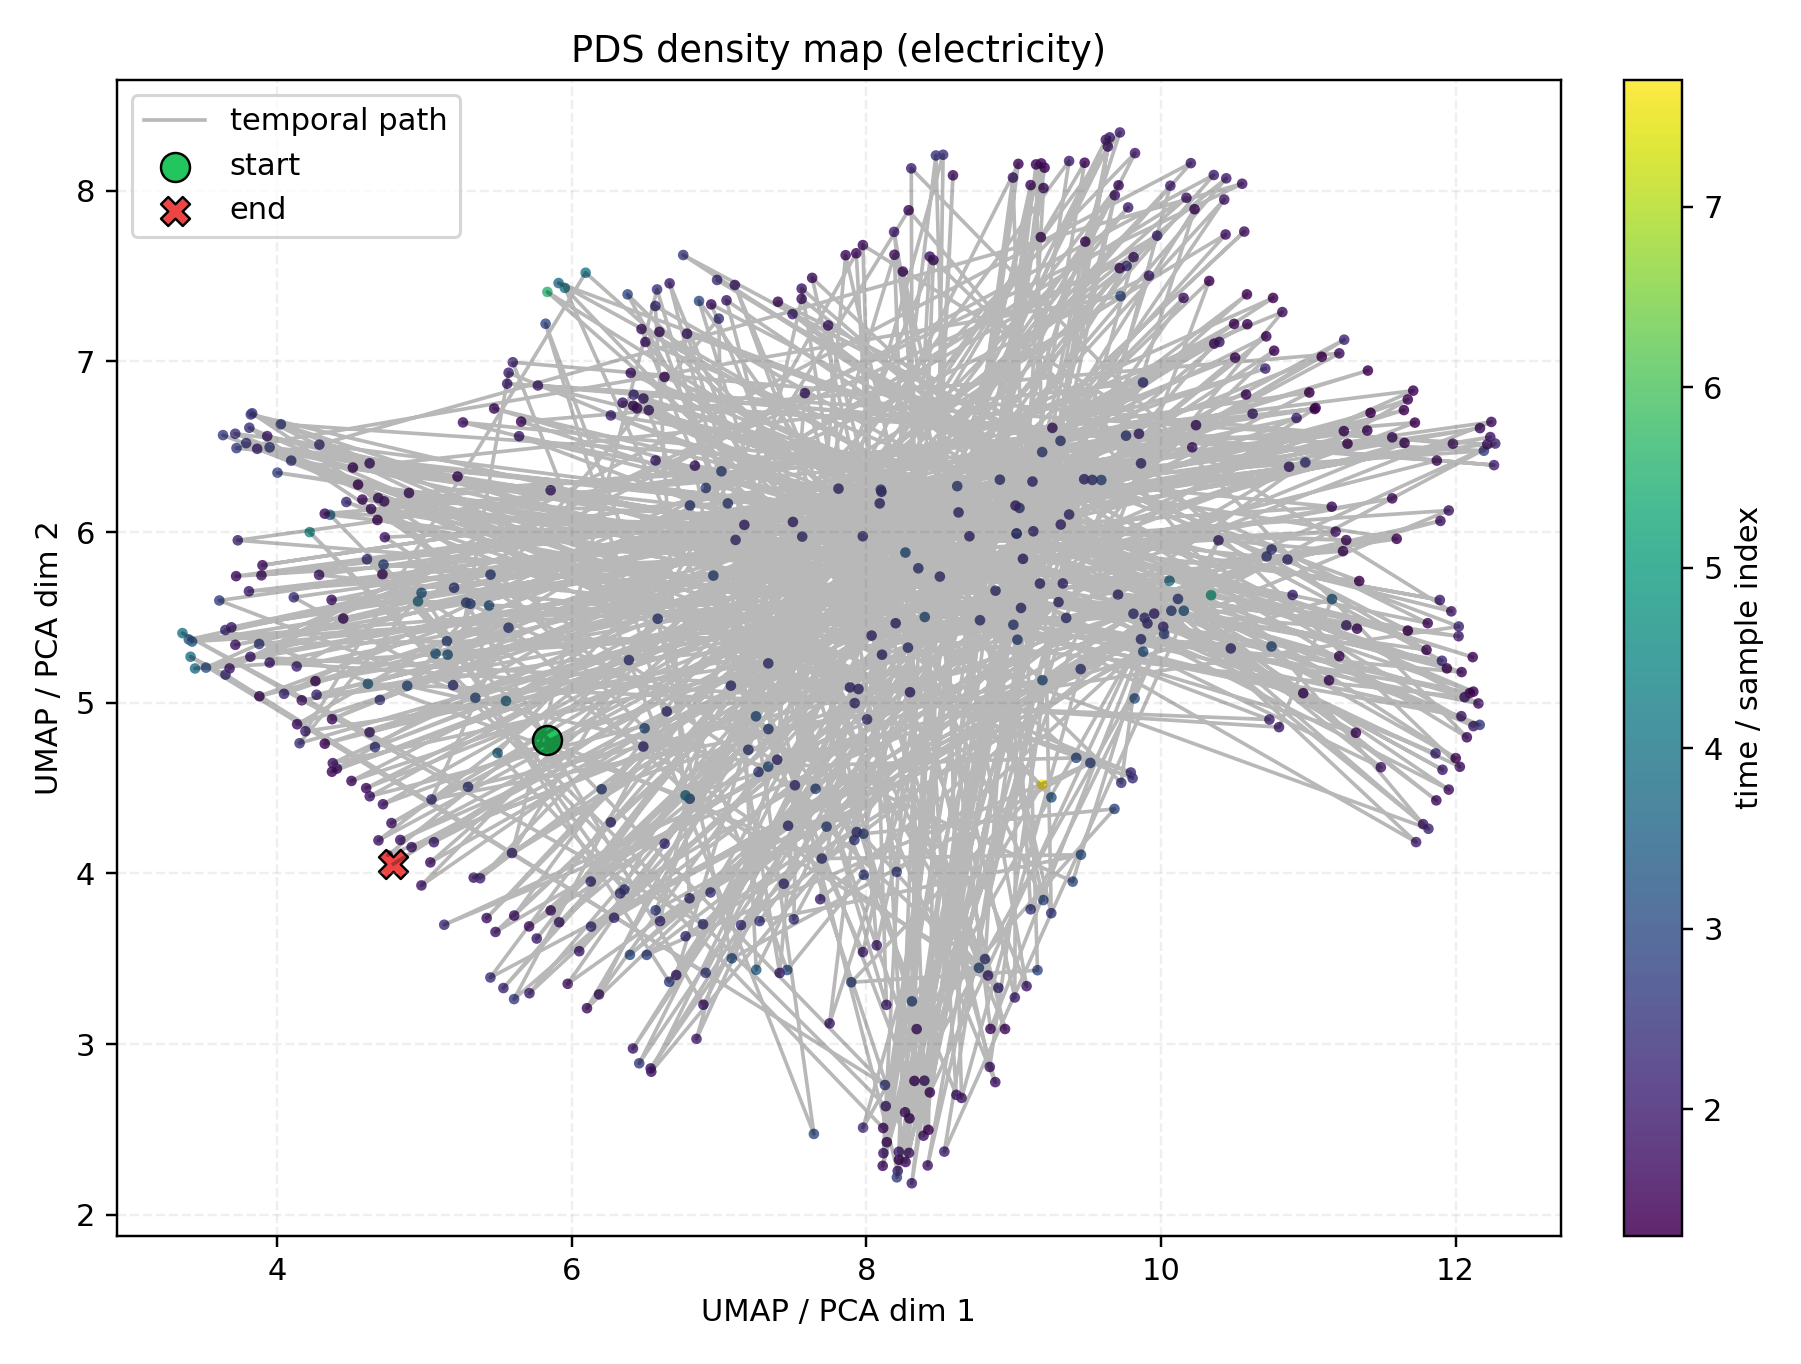
\includegraphics[width=\linewidth]{fig_pds_density_elec}\\[2pt]
  \small\textbf{(a) Electricity (in-distribution)}
\end{minipage}
\hfill
\begin{minipage}[b]{0.43\linewidth}
  \centering
  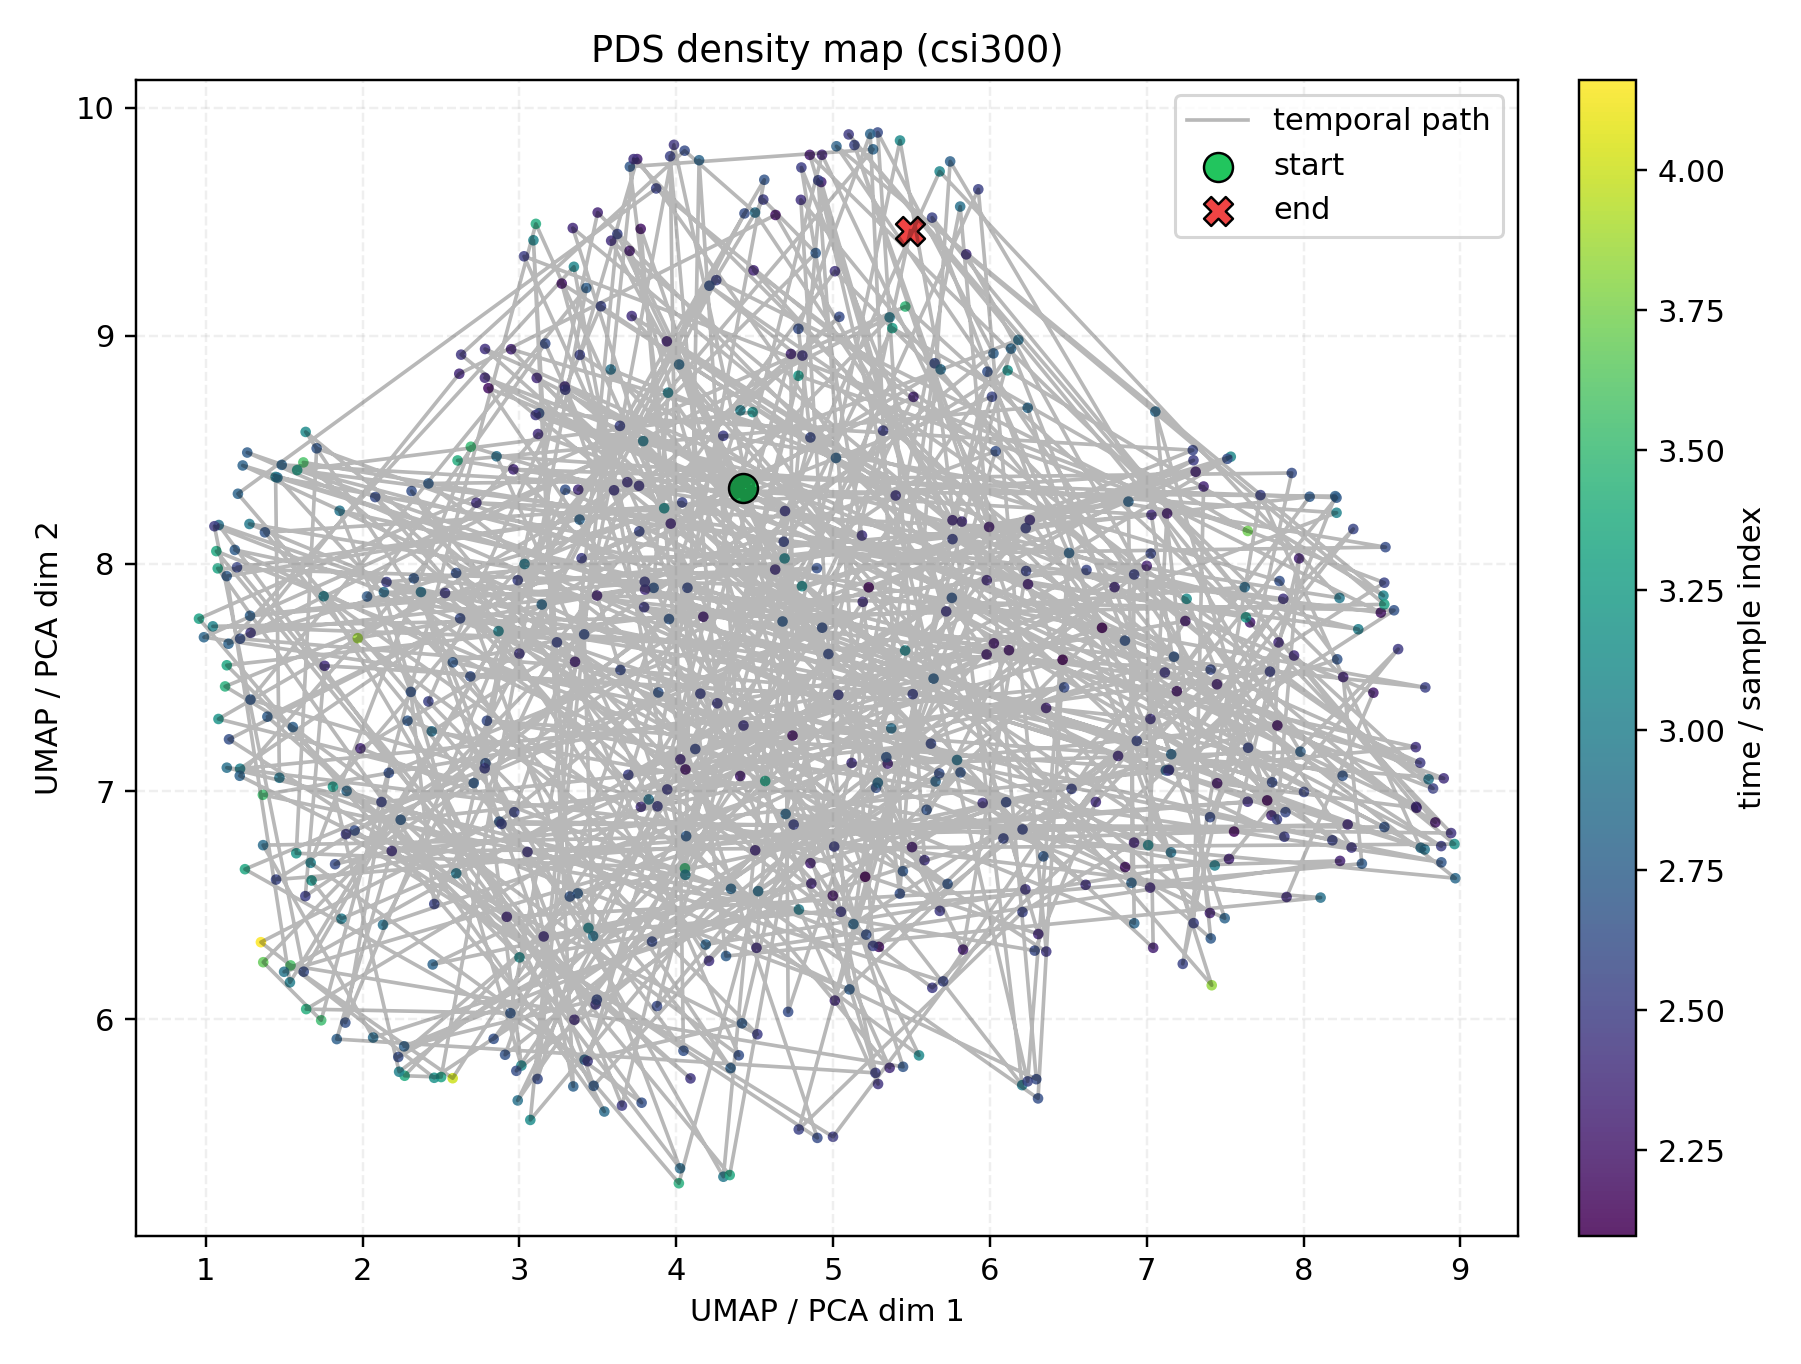
\includegraphics[width=\linewidth]{fig_pds_density_csi300}\\[2pt]
  \small\textbf{(b) CSI300 (OOD equity)}
\end{minipage}
\caption{\textbf{Neighbourhood isolation maps explaining PDS transfer vs.\ collapse.}
  Points show UMAP projections; colour encodes mean $k$-NN distance
  $\bar{d}_i$ computed in the full 1{,}024-D embedding space (the
  figure's colorbar reads ``time / sample index''---a display artefact
  from the shared visualisation function; values here are $\bar{d}_i$).
  The key difference is in the colour range, not the cloud shape:
  on Electricity (a), $\bar{d}_i$ spans ${\approx}2$--$7$ (range $\approx 5$),
  creating the density contrast that yields $\rspear^{\pds}{=}0.41$
  ($p{<}10^{-20}$).
  On OOD CSI300 (b), the range compresses to ${\approx}2.25$--$4.0$
  (range $\approx 1.75$): OOD windows distribute near-uniformly across the
  manifold, eliminating variance in $\bar{d}_i$ and driving
  $\rspear^{\pds}$ to $0.02$ ($p{>}0.3$), exactly as
  Theorem~\ref{thm:pds_main}(ii) predicts.}
\label{fig:pds_density_comparison}
\end{figure}
\FloatBarrier

% =====================================================================
\section{Conclusion}
\label{sec:conclusion}
% =====================================================================

LGF reveals a compact, selective, and distribution-bounded geometric imprint
from pretraining.
TimesFM's manifold sits $3.5\times$ below the supervised Transformer
($\ltcstep{=}4.64$ vs.\ $16.16$) yet $19\%$ above the random-weight encoder,
with lower intrinsic dimension directly tightening prediction risk.
Frozen embeddings encode seasonality ($78.6\%$) and volatility ($70.9\%$)
well above chance but not trend direction, which window-level normalisation
provably erases.
Neighbourhood reliability (PDS) holds within distribution ($\rho{=}0.41$) but
collapses on OOD equity ($\rho{\approx}0$)---a three-way split confirmed across
all ten external TSFMs.
The ETTh1 memorisation signature ($\ltcstep{>}15$ for OFA, UniTime, TiRex,
Moirai) is invisible to forecasting metrics, demonstrating diagnostic value
beyond held-out loss.
Priority extensions: random-weight controls and CSS probing for MOMENT, Moirai,
and Chronos; connecting geometry to scaling laws \citep{edwards2024scalinglaws}
and leakage-controlled benchmarks \citep{aksu2024gifteval,qiu2024tfb}.
\textbf{Limitations:} all geometry--forecast correlations are observational
(causal claims require architecture ablations); random-weight controls are
currently available only for TimesFM~2.0.
\label{sec:limitations}

% =====================================================================
\bibliographystyle{plainnat}
\bibliography{refs}
% =====================================================================

% =====================================================================
%                        APPENDIX
% =====================================================================
\appendix

% =====================================================================
\section{Extended Related Work}
\label{app:related_full}
% =====================================================================

\paragraph{Time series foundation models.}
The TSFM landscape has diversified across several architectural paradigms
\citep{liang2024foundation,jin2023large,meyer2025tsfmreview}.
\emph{Encoder-decoder masked pretraining}: MOMENT \citep{goswami2024moment}
and Moirai \citep{woo2024moirai} learn via masked patch reconstruction;
Moirai-MoE \citep{woo2024moiraimoe} extends with sparse mixture-of-experts.
\emph{Decoder-only autoregressive}: TimesFM \citep{das2024timesfm} and Timer
\citep{liu2024timer} treat forecasting as next-patch prediction.
\emph{Language-model-inspired}: Chronos \citep{ansari2024chronos} quantises
values into tokens and fine-tunes T5; Lag-Llama \citep{rasul2024lagllama}
adapts Llama for probabilistic forecasting; LLMTime \citep{gruver2023llmts}
prompts frozen LLMs.
\emph{Efficient}: Time-MoE \citep{shi2024timemoe} scales to billions of
parameters.
\citet{edwards2024scalinglaws} established predictable TSFM scaling laws.

\paragraph{Evaluation integrity and benchmarking.}
Leakage concerns \citep{meyer2025tsfmreview} arise because Electricity and
ETTh1 appear verbatim in multiple pretraining corpora.
GIFT-Eval \citep{aksu2024gifteval}, TSFM-Bench \citep{li2025tsfmbench}, and
TFB \citep{qiu2024tfb} address this; CSI300 and CSI800 provide a
leakage-free geometric test.

\paragraph{Geometric analysis of representations.}
\citet{ansuini2019intrinsic} established layer-wise intrinsic dimensionality
profiles for image classifiers; \citet{aghajanyan2021intrinsic} connected low
intrinsic dimension to efficient adaptation.
\citet{reif2019visualizing} characterised BERT's syntactic geometry;
\citet{raghu2017svcca} used SVCCA to track representation formation.
None of this work addresses time series.

\paragraph{Explainability for time series.}
XAI methods \citep{ismail2020benchmarking,theissler2022explainable} assign
input-level importance scores via LIME, SHAP, or integrated gradients.
Linear probing \citep{alain2017probing} tests concept readability from frozen
representations---the basis for CSS.

% =====================================================================
\section{LGF Framework: Intuition and Supporting Figures}
\label{app:framework_figs}
% =====================================================================

\subsection{LTC: Temporal Trajectory Complexity}
\label{app:ltc_fig}

LTC treats the sequence of frozen embeddings as a path through $\R^D$ and
measures its arc length ($\ltcstep$) and directionality ($\ltcdir$).
Figure~\ref{fig:ltc_intuition} illustrates the contrast: a random encoder
produces short, undirected steps ($\ltcdir{\approx}0$); a pretrained encoder
produces a longer, consistently-directed path.

\begin{figure}[h]
\centering

\includegraphics[width=\linewidth]{fig_ltc_intuition}
\caption{LTC intuition (schematic, 2D projection).
\emph{Left}: random encoder---short, undirected steps.
\emph{Right}: pretrained encoder---longer, directionally consistent path.}
\label{fig:ltc_intuition}
\end{figure}

Figure~\ref{fig:ltc_profile} (main text) places quantitative results in
perspective.
Pretrained TimesFM~2.0 consistently exceeds its random-weight control on
every dataset (confirming Proposition~\ref{prop:ltc_pretraining}), and
$\ltcstep$ varies with dataset structure: high-frequency Electricity and
heterogeneous Traffic produce denser trajectories than Weather.
The supervised Transformer achieves $\ltcstep{=}16.2$ on Electricity---$3.5\times$
larger than TimesFM ($4.64$)---yet this does not translate to better forecasts,
showing pretraining selects for a compact, structured manifold rather than a
maximally complex one.

\subsection{Manifold Regularity: LCS Cluster Structure}
\label{app:reg_figs}

LCS measures whether same-trend embeddings form distinct spatial regions.
Figure~\ref{fig:lcs_clusters} contrasts the pretrained encoder (positive LCS,
compact trend clusters) with the random-weight control (LCS $\approx 0$,
intermixed cloud), consistent with Proposition~\ref{prop:lcs_degenerate}.
A positive LCS certifies actively learned structure: in high dimensions,
i.i.d.\ random embeddings produce $\E[\lcs] \to 0$ regardless of model
quality.

\begin{figure}[h]
\centering

\includegraphics[width=\linewidth]{fig_lcs_clusters}
\caption{\textbf{LCS cluster organisation (2D PCA projection, schematic illustration).}
The figure titles display \texttt{LCS = 0.000} for both panels; this is a
visualisation artefact from the schematic rendering, not a result from the
held-out benchmarks.
The schematic shows the concept: same-trend embeddings occupy distinct
spatial regions in a well-organised embedding space (left, pretrained) vs.\
an intermixed cloud (right, random control).
Empirical LCS values for pretrained TimesFM are positive on Traffic and
Weather; ablation results are in Appendix~\ref{app:ablations}.}
\label{fig:lcs_clusters}
\end{figure}

\subsection{Reliability: PDS vs.\ FSS Concept}
\label{app:rel_fig}

PDS correlates $k$-NN isolation $\bar{d}_i$ with per-window forecast error;
FSS correlates pairwise embedding distance with pairwise error difference.
Figure~\ref{fig:pds_concept} illustrates why they differ: PDS detects local
density variation; FSS requires global monotonicity between distance and
error, which fails whenever the manifold has both dense and sparse regions
at similar global scales.
On OOD data, all embeddings land in uniformly sparse regions, eliminating
local variance and collapsing PDS to near zero
(Theorem~\ref{thm:pds_main}(ii)).

\begin{figure}[h]
\centering

\includegraphics[width=\linewidth]{fig_pds_concept}
\caption{PDS and FSS concepts (schematic).
\emph{Left}: isolated embeddings predict larger errors; OOD collapse occurs
when all points are equally isolated.
\emph{Right}: global pairwise distances miss local density structure.}
\label{fig:pds_concept}
\end{figure}

\subsection{PDS vs.\ FSS Per Dataset}
\label{app:geodesic_fig}

Figure~\ref{fig:geodesic} (main text) shows PDS--FSS per dataset at the
average horizon.
On Electricity, PDS substantially exceeds FSS ($\Delta\rho{=}0.40$), driven
by pronounced local density variation.
Traffic shows a similar but smaller gap ($\Delta\rho{=}0.20$).
Weather and ETTh1 show weaker signals: the outlier cluster in Weather
disrupts the in-distribution density gradient, while ETTh1's
memorisation-level trajectory compresses all windows into a narrow band.
The random-weight control is consistently near zero or negative, confirming
that positive PDS requires learned manifold structure.

\subsection{CSS Probing: Decoding Temporal Concepts}
\label{app:css_fig}

We probe three STL-derived binary concepts: trend direction, seasonal phase,
and volatility, using an $\ell_2$-regularised logistic probe (80/20
train/test split, permutation tests $n_{\mathrm{perm}}{=}60$ for
in-distribution, $n_{\mathrm{perm}}{=}20$ for OOD, per
Proposition~\ref{prop:permtest_app}).
Figure~\ref{fig:css_probe} shows the three scenarios: seasonality and
volatility produce clearly separable linear boundaries; trend does not,
consistent with Theorem~\ref{thm:css_main}(i) and window-level
normalisation.

\begin{figure}[h]
\centering

\includegraphics[width=\linewidth]{fig_css_probe}
\caption{CSS linear probing (schematic 2D PCA projection).
\emph{Left/Centre}: seasonality and volatility produce above-chance linear
separation.
\emph{Right}: trend produces no separable boundary, consistent with
Theorem~\ref{thm:css_main}(i).}
\label{fig:css_probe}
\end{figure}

\subsection{OOD Validation: Three-Way Metric Split}
\label{app:ood_fig}

The OOD prediction (Theorem~\ref{thm:pds_main}(ii)) is stated before any
equity data is examined, providing genuine pre-registration.
Figure~\ref{fig:ood_summary} (main text) shows the three-way split: pretrained
LTC exceeds the random control on both equity datasets; CSS (seasonality) is
above chance on both; PDS collapses to near-zero on both.
This transfer/transfer/collapse pattern is the most direct evidence that LGF
metrics diagnose qualitatively distinct properties of the learned
representation.
Figure~\ref{fig:pds_density_comparison} (main text) provides the geometric
explanation: OOD embeddings fill the manifold uniformly, eliminating the
density variation that PDS requires.

\subsection{Ablation Studies}
\label{app:ablations}

$\rspear^{\pds}$ remains positive and significant for $k\in\{10,20,50\}$ on
Electricity ($\rho{>}0.15$).
LCS directional rankings (pretrained $\geq$ random on Weather and Traffic)
hold across STL slope thresholds $\delta\in\{0.02,0.05,0.10\}$.
The $\ltcstep$ advantage of pretrained over random persists at all four
horizons $H\in\{96,192,336,720\}$.

\subsubsection*{Full 14-model LTC and PDS/FSS results}

\begin{table}[h]
\centering
\caption{\textbf{Full $\ltcstep$ results for all 14 TSFMs.}
Supplement to Table~\ref{tab:ltc} (main text). \textbf{Bold}: ETTh1 $>15$.}
\label{tab:ltc_ext}
\small
\setlength{\tabcolsep}{3pt}
\begin{tabular}{lccccr}
\toprule
\textbf{Model} & \textbf{Elec.} & \textbf{Weath.} & \textbf{ETTh1} & \textbf{Traffic} & $\Delta$\\
\midrule
TimesFM (pre)  & 4.64 & 5.10 & 5.02 & 3.77 & $+$1.21\\
TimesFM (rand) & 3.90 & 3.52 & 3.70 & 2.55 & ---\\
$\Delta$       & +0.74 & +1.58 & +1.32 & +1.22 & \\
\midrule
LSTM           &  4.75 & --- & --- & --- & ---\\
TCN            &  5.56 & --- & --- & --- & ---\\
Transformer    & 16.16 & --- & --- & --- & ---\\
\midrule
\multicolumn{6}{l}{\textit{Additional TSFMs (no random-weight control)}}\\
LightGTS      & 1.59 & 0.64 & 8.86  & 1.63 & ---\\
OFA           & 1.00 & 1.68 & \textbf{17.69} & 1.62 & ---\\
Sundial       & 4.00 & 5.60 & 3.00  & 6.77 & ---\\
Time-MoE      & 0.77 & 1.40 & 4.09  & 1.77 & ---\\
UniTime       & 3.30 & 2.68 & \textbf{28.90} & 3.86 & ---\\
VisionTS      & 0.99 & 0.62 & 6.11  & 1.20 & ---\\
TiRex         & 9.62 & 2.82 & \textbf{25.53} & 8.89 & ---\\
MOMENT-Large  & 2.03 & 1.98 & 2.16  & 2.82 & ---\\
Moirai        & 9.97 & 2.91 & \textbf{26.66} & 9.64 & ---\\
Chronos-Small & 0.13 & 0.19 & 0.21  & 0.15 & ---\\
\bottomrule
\end{tabular}
\end{table}

\begin{table}[h]
\centering
\caption{\textbf{Full PDS/FSS results for all additional TSFMs.}
Supplement to Table~\ref{tab:geodesic} (main text).
$^\dagger$ $p{>}0.05$. $^\ddagger$ driven by ETTh1. $^\S$ ETTh1-dominated.}
\label{tab:geodesic_ext}
\small
\setlength{\tabcolsep}{3pt}
\begin{tabular}{lcc}
\toprule
\textbf{Model} & $\rspear^{\pds}$ (4-ds mean) & $\rspear^{\fss}$ (4-ds mean)\\
\midrule
LightGTS      & $-0.17^\dagger$ & $-0.76$\\
OFA           & $-0.12^\dagger$ & $-0.95$\\
Sundial       & $+0.24^{\S}$    & $-0.40$\\
Time-MoE      & $+0.13^{\S}$    & $-0.24$\\
UniTime       & $-0.19^\dagger$ & $-0.71$\\
VisionTS      & $-0.13^\dagger$ & $-0.54$\\
TiRex         & $-0.15^\dagger$ & $-0.64$\\
MOMENT-Large  & $-0.10^\dagger$ & $-0.20$\\
Moirai        & $-0.15^\dagger$ & $-0.63$\\
Chronos-Small & $+0.08^\ddagger$& $-0.15$\\
\midrule
OOD equity (CSI300+CSI800 mean) & $[-0.29,\,-0.01]$ & $[-0.56,\,-0.20]$\\
\bottomrule
\end{tabular}
\end{table}
Appendix~\ref{app:horizon_pds} shows that the positive PDS signal on
Electricity and Traffic is maintained at all four horizons and is not an
artefact of averaging.

\subsection{Limitations and Future Directions}
\label{app:limitations}

LGF has been empirically evaluated on four architectures (TimesFM~2.0,
MOMENT-Large, Moirai, Chronos-Small); state-space and vision-based TSFMs
remain outstanding extensions.
Random-weight controls and CSS probing are available only for TimesFM~2.0,
so cross-architecture comparisons lack the pretrained-vs-random contrast.
Three of four main benchmarks may overlap TSFM pretraining corpora; Traffic
and the equity indices are more reliable.
All correlations are observational.

Immediate priorities: CSS probing for MOMENT, Moirai, and Chronos;
random-weight controls for these models; leakage-controlled benchmarks
\citep{aksu2024gifteval,qiu2024tfb}; and connecting geometric richness to
scaling laws \citep{edwards2024scalinglaws}.

% =====================================================================
\section{Full Theoretical Proofs}
\label{app:proofs}
% =====================================================================

\subsection{Manifold Foundations}
\label{app:manifold_proofs}

\begin{theorem}[TRM Compactness and Rectifiability]
\label{thm:trm_rect_app}
Under Assumption~\ref{asm:lipschitz} and compact input support, $\trm$ is
compact and rectifiable: it has finite Hausdorff measure and can be covered
by finitely many Lipschitz images of bounded subsets of $\R^d$, $d \leq L$.
\end{theorem}
\begin{proof}
The continuous image of a compact set under a Lipschitz map is compact.
By Rademacher's theorem, $f_\theta$ is differentiable almost everywhere with
Jacobian of rank $\leq \min(L,D)$.
By Federer's structure theorem \citep{federer1969geometric}, the image is
countably $m$-rectifiable for $m \leq L$; compactness reduces this to a
finite cover.
\end{proof}

\begin{theorem}[Intrinsic Dimension Bound]
\label{thm:id_bound_app}
For $\mathcal{P}$-almost every window $w$, the local dimension of $\trm$
at $z = f_\theta(w)$ satisfies
$\dint(z) \leq \mathrm{rank}(J_{f_\theta}(w)) \leq \min(L,D)$.
\end{theorem}
\begin{proof}
By the rank theorem, the tangent space of $\trm$ at $z$ is contained in the
image of $\mathrm{d}f_\theta|_w$, which has dimension $\mathrm{rank}(J_{f_\theta}(w))$.
\end{proof}

\begin{theorem}[Concentration of Pairwise Distances]
\label{thm:concentration_app}
For i.i.d.\ draws from a spherically symmetric distribution on
$S^{D-1}(\sqrt{D})$, for any $\epsilon > 0$:
\[
  \Prob\!\left(\abs{\norm{z_i - z_j}_2 - \sqrt{2D}} > \epsilon\sqrt{D}\right)
  \leq 2\exp(-c_0\epsilon^2 D).
\]
\end{theorem}
\begin{proof}
$g(z) = \norm{z - z_j}_2$ is $1$-Lipschitz. L\'{e}vy's lemma for
$S^{D-1}(\sqrt{D})$ \citep{ledoux2001concentration} gives
$\Prob(|g(z) - M_g| > t) \leq 2\exp(-{(D-1)t^2}/{(2D)})$.
The expected distance is $\sqrt{2D}(1+O(1/D))$; set $t = \epsilon\sqrt{D}$.
\end{proof}

\begin{proposition}[LCS Degeneracy for Random Embeddings]
\label{prop:lcs_degenerate}
For i.i.d.\ random embeddings on $S^{D-1}(\sqrt{D})$,
$\E[\lcs] \to 0$ as $D \to \infty$.
\end{proposition}

\begin{proof}[Proof of Proposition~\ref{prop:lcs_degenerate}]
By Theorem~\ref{thm:concentration_app}, all pairwise distances concentrate
around $\sqrt{2D}$.
The silhouette numerator $b(i)-a(i) = O(\epsilon\sqrt{D})$ while the
denominator $\max(a(i),b(i)) = \Theta(\sqrt{D})$, giving
$\E[\lcs] = O(\epsilon) \to 0$ for any fixed $\epsilon$.
\end{proof}

% ---------------------------------------------------------------
\subsection{LTC Proofs}
\label{app:ltc_proofs}

\begin{proposition}[LTC$_{\mathrm{step}}$ as Arc Length]
\label{prop:ltc_arc}
$\ltcstep$ equals the normalised arc length of the piecewise-linear temporal
trajectory through $\Zset$.
$\ltcdir = 1$ iff all consecutive steps are parallel (perfectly straight
trajectory); $\ltcdir \approx 0$ corresponds to a random walk in embedding space.
\end{proposition}

\begin{proposition}[Pretraining Amplifies LTC$_{\mathrm{step}}$]
\label{prop:ltc_pretraining}
Under Assumption~\ref{asm:lipschitz} and ergodic temporal variation,
if the pretraining objective requires sensitivity to temporal context, then
$\E[\ltcstep(f_\theta)] \geq \E[\ltcstep(f_{\theta_0})]$
for any randomly-initialised control $f_{\theta_0}$.
\end{proposition}

\begin{proof}[Proof of Proposition~\ref{prop:ltc_arc}]
The piecewise linear temporal trajectory $\Gamma_N$ has segments $\delta_i$.
Its arc length is $\sum_{i=1}^{N-1}\norm{\delta_i}_2 = (N-1)\ltcstep$ by
definition.
$\ltcdir = 1$ iff every cosine similarity $\delta_i\cdot\delta_{i+1}/
(\norm{\delta_i}\norm{\delta_{i+1}}) = 1$, which holds iff all consecutive
steps are positively proportional (Cauchy-Schwarz equality condition).
For i.i.d.\ uniform steps on $S^{D-1}$, $\E[\ltcdir] = 0$ for $D\geq 2$.
\end{proof}

\begin{proof}[Proof of Proposition~\ref{prop:ltc_pretraining}]
$\E[\ltcstep(f_\theta)] = (N-1)^{-1}\sum_i\E[\norm{f_\theta(w_{\sigma(i+1)})
- f_\theta(w_{\sigma(i)})}_2]$.
An autoregressive/masked pretraining objective requires the encoder to
distinguish temporal contexts; specifically,
$\E[f_\theta(w_{t+1}) \neq f_\theta(w_t)]$ is non-trivial, so the expected
displacement is positive along the most sensitive direction.
For $f_{\theta_0}$ with random weights, parameters are independent of data,
so the expected displacement is governed only by data variation
$\E[\norm{w_{t+1}-w_t}_2]$ filtered through untrained weights, which is
no larger than the pretrained case when the objective provides meaningful
updates.
\end{proof}

% ---------------------------------------------------------------
\subsection{Lipschitz Stability Proofs}
\label{app:stability_proofs}

\begin{lemma}[Residual Connection]
\label{lem:residual_app}
If $F$ is $L_F$-Lipschitz, then $h(x) = x + F(x)$ is $(1+L_F)$-Lipschitz.
\end{lemma}
\begin{proof}
$\norm{h(x)-h(y)}_2 \leq \norm{x-y}_2 + \norm{F(x)-F(y)}_2
\leq (1+L_F)\norm{x-y}_2$.
\end{proof}

\begin{theorem}[Transformer Lipschitz Constant]
\label{thm:transformer_lip_app}
An $\mathcal{L}$-layer Transformer encoder has Lipschitz constant at most
\[
  L_\theta \leq \prod_{\ell=1}^{\mathcal{L}}
  (1+\smax(W_O^\ell)\smax(W_V^\ell))
  (1+\smax(W_2^\ell)\smax(W_1^\ell)).
\]
\end{theorem}
\begin{proof}
For a frozen attention weight matrix $A$ (row-stochastic, $\norm{A}_2\leq 1$),
$\Lip(\mathrm{MSA}) \leq \smax(W_O)\smax(W_V)$.
By Lemma~\ref{lem:residual_app}, the residual self-attention sub-block is
$(1+\smax(W_O^\ell)\smax(W_V^\ell))$-Lipschitz.
The FFN with $1$-Lipschitz activation is $(\smax(W_2)\smax(W_1))$-Lipschitz;
its residual sub-block adds $1$.
The full encoder is a composition of $\mathcal{L}$ such layers.
\end{proof}

\begin{proof}[Proof of Theorem~\ref{thm:tsi_main}]
Write $\tilde{z}_i = z_i + \Delta_i$, $\norm{\Delta_i}_2 \leq L_\theta\epsilon$.
The cosine similarity for window $i$:
\[
  \frac{z_i\cdot\tilde{z}_i}{\norm{z_i}\norm{\tilde{z}_i}}
  = \frac{\norm{z_i}^2 + z_i\cdot\Delta_i}{\norm{z_i}\norm{z_i+\Delta_i}}
  \geq \frac{\mu^2 - \mu L_\theta\epsilon}{\mu(\mu + L_\theta\epsilon)}
  = \frac{\mu - L_\theta\epsilon}{\mu + L_\theta\epsilon},
\]
using $z_i\cdot\Delta_i \geq -\norm{z_i}L_\theta\epsilon$ (Cauchy-Schwarz)
and $\norm{z_i+\Delta_i} \leq \norm{z_i} + L_\theta\epsilon$ (triangle).
Averaging over $i$ preserves the inequality.
\end{proof}

\begin{theorem}[GSP Controlled by TSI Deficit]
\label{thm:gsp_bound_app}
If $\tsi_{\mathcal{P}} \geq 1-\kappa$ and $\norm{z_i}_2 \leq R$, then
$\abs{\gsp_{\mathcal{P}}} \leq 4R\kappa^{1/2}/\bar{d}$,
where $\bar{d}$ is the mean pairwise embedding distance.
\end{theorem}
\begin{proof}
$\tsi \geq 1-\kappa$ implies average perturbation $\E[\norm{\Delta_i}_2]
\leq 2R\kappa^{1/2}$ (from the angle-to-distance bound
$\norm{\Delta} \leq 2R\sin(\theta/2) \leq R\theta \leq 2R\kappa^{1/2}$).
The silhouette score changes are bounded by perturbation size divided by
mean pairwise distance $\bar{d}$:
$\abs{\lcs_{\mathrm{clean}}-\lcs_{\mathcal{P}}} \leq 4R\kappa^{1/2}/\bar{d}$.
\end{proof}

% ---------------------------------------------------------------
\subsection{CSS and Linear Probing Proofs}
\label{app:probing_proofs}

\begin{proof}[Proof of Theorem~\ref{thm:css_main}]
\textbf{(i)} The balanced accuracy of an optimal linear classifier exceeds
$1/2$ iff the class means are distinct in the Mahalanobis metric, i.e.,
Fisher discriminant ratio $J_F = (\mu_+-\mu_-)^\top\Sigma^{-1}(\mu_+-\mu_-)
> 0$.

\textbf{(ii)} The logistic regression probe achieves error rate $P_e = 1-\alpha$.
By Fano's inequality: $H(Y^c | Z) \leq \Hb(P_e) = \Hb(1-\alpha)$.
With balanced binary labels $H(Y^c) = 1$ bit:
$I(Z;Y^c) = H(Y^c) - H(Y^c|Z) \geq 1 - \Hb(1-\alpha)$.

\textbf{(iii)} Applying (ii) to both pretrained ($\alpha_p$) and random
($\alpha_r$) and taking the difference:
$I(Z_\theta;Y^c) - I(Z_{\theta_0};Y^c) \geq \Hb(1-\alpha_r) - \Hb(1-\alpha_p)$.
Since $\alpha_p > \alpha_r$ and $\Hb$ is decreasing on $(1/2, 1)$, the
right-hand side is positive.
\end{proof}

\begin{proposition}[Permutation Test Validity]
\label{prop:permtest_app}
Under $H_0: Z \perp Y^c$, the permutation test p-value
$\hat{p} = (1 + \sum_j\mathbf{1}[\css_j \geq \css_{\mathrm{obs}}])/(n_{\mathrm{perm}}+1)$
controls Type~I error at level $\alpha$ for any
$\alpha \geq 1/(n_{\mathrm{perm}}+1)$.
\end{proposition}
\begin{proof}
Under $H_0$, the label vector is exchangeable under permutation.
$\css_{\mathrm{obs}}$ is uniformly distributed among $n_{\mathrm{perm}}+1$
exchangeable values, so $\Prob_{H_0}(\hat{p} \leq \alpha) \leq \alpha$.
\end{proof}

% ---------------------------------------------------------------
\subsection{Reliability Geometry Proofs}
\label{app:reliability_proofs}

\begin{theorem}[k-NN Distance and Manifold Density]
\label{thm:knn_density_app}
For i.i.d.\ draws from density $\rho$ on a smooth $\dint$-dimensional
manifold, the mean $k$-nearest-neighbour distance satisfies
$\bar{d}_i^{(k)} \approx c_{\dint,k}\,\rho(z_i)^{-1/\dint}$
as $N\to\infty$, where
$c_{\dint,k} = (\Gamma(\dint/2+1)/(\pi^{\dint/2}k))^{1/\dint}$.
\end{theorem}
\begin{proof}
In a locally flat region of density $\rho$, the expected number of points
within radius $r$ is $N\rho(z_i)\omega_{\dint}r^{\dint}$.
Setting this to $k$ gives
$r_k \approx (k/(N\rho\omega_{\dint}))^{1/\dint}$, from which the mean
$k$-NN distance follows immediately.
See \citet{penrose2003random} for the full proof via empirical process theory.
\end{proof}

\begin{proof}[Proof of Theorem~\ref{thm:pds_main}]
\textbf{(i)} Both $\bar{d}_i$ and $|e_i|$ are non-decreasing in the same
distributional-shift measure, so their ranks are concordant in expectation
and $\rspear^{\pds} \geq 0$ by Kendall's $\tau \geq 0$.

\textbf{(ii)} For OOD test data, $\rho(z_i)$ is uniformly low (all embeddings
in sparse regions), so $\bar{d}_i$ has low variance. The Spearman correlation
of a near-constant sequence with any other is near zero.

\textbf{(iii)} Construct two clusters: dense $A$ with low error, sparse $B$
with high error, globally close but locally distinct.
Global pairwise distances (FSS) cannot distinguish A-A from A-B pairs
(similar means), so $\rspear^{\fss} \approx 0$.
Local k-NN distances (PDS) correctly assign high $\bar{d}$ to $B$-points,
giving high $\rspear^{\pds}$.
The ratio $\sigma_B/\sigma_A$ can be made arbitrarily large, showing
$\rspear^{\pds} \gg \rspear^{\fss}$ is achievable.
\end{proof}

% ---------------------------------------------------------------
\subsection{Generalisation Bounds}
\label{app:gen_proofs}

\begin{theorem}[Covering Number of TRM]
\label{thm:covering_app}
Under Assumption~\ref{asm:lipschitz} and compact support of radius $R_w$:
\[
  \mathcal{N}(\trm,\norm{\cdot}_2, \epsilon)
  \leq \left(\frac{2L_\theta R_w}{\epsilon}\right)^{\dint}.
\]
\end{theorem}
\begin{proof}
The input support has an $\delta$-cover of size $(2R_w/\delta)^L$.
Mapping through the $L_\theta$-Lipschitz encoder magnifies radius by
$L_\theta$; setting $L_\theta\delta = \epsilon/2$ and using
$\dint \leq L$ gives the bound.
\end{proof}

\begin{theorem}[Generalisation Bound from Manifold Complexity]
\label{thm:gen_bound_app}
Let $\mathcal{F}$ be $G$-Lipschitz predictors with $|\hat{e}| \leq M$ on
$\trm$. With probability $1-\delta$:
\[
  \sup_{\hat{e}}|L(\hat{e}) - \hat{L}_N(\hat{e})|
  \leq 2GM\sqrt{\frac{\dint\log(2L_\theta R_w/\epsilon)}{N}}
  + 3M\sqrt{\frac{\log(2/\delta)}{2N}}.
\]
\end{theorem}
\begin{proof}
The Rademacher complexity of Lipschitz functions on a compact set is bounded
by $\sqrt{\log\mathcal{N}(\trm,\epsilon)/N} + O(\epsilon)$
\citep{shalev2014understanding}.
Substituting Theorem~\ref{thm:covering_app} and optimising over $\epsilon$
gives the result.
\end{proof}

\begin{corollary}[Compact TRM Implies Tighter OOD Generalisation]
\label{cor:low_id_app}
If $f_{\theta_1}$ has $\dint^{(1)} < \dint^{(2)}$ but the same empirical
risk as $f_{\theta_2}$, then $f_{\theta_1}$ has a tighter generalisation
bound by factor $\sqrt{\dint^{(1)}/\dint^{(2)}}$.
\end{corollary}

% =====================================================================
\section{Extended Experimental Details}
\label{app:exp_details}
% =====================================================================

\subsection{Datasets}

\begin{table}[h]
\centering
\caption{Datasets used in LGF analysis. CSI300/CSI800 are OOD validation only.}
\label{tab:datasets}
\small
\setlength{\tabcolsep}{6pt}
\begin{tabular}{llrl}
\toprule
\textbf{Dataset} & \textbf{Domain} & \textbf{Length} & \textbf{Freq.}\\
\midrule
Electricity & Energy       & 26{,}304 & Hourly \\
ETTh1       & Temperature  & 17{,}420 & Hourly \\
Weather     & Meteorology  & 52{,}696 & 10-min \\
Traffic     & Flow         & 34{,}272 & 5-min  \\
\midrule
CSI300      & Equity (OOD) & 58{,}600 & Daily  \\
CSI800      & Equity (OOD) & 58{,}600 & Daily  \\
\bottomrule
\end{tabular}
\end{table}

\subsection{Hyperparameters and Implementation}

\paragraph{Window extraction.}
$N=3{,}000$ sliding windows, length $L=512$, stride $64$.
Each window is normalised to zero mean and unit variance.
Start times $s_i$ recorded for LTC computation.

\paragraph{Embedding extraction.}
\textbf{TimesFM~2.0}: patch size $P=32$, $T=16$ patch tokens per window,
$D=1{,}024$.
Chronos-Small uses T5-Small encoder last-layer hidden states mean-pooled to
$D=512$; MOMENT-Large uses patch size $P=16$, $D=1{,}024$; Moirai uses
last-layer mean-pooled hidden states at $D=768$.

\paragraph{PDS and FSS.}
$k$-NN graph with Euclidean metric; $k=10$
($k\in\{10,20,50\}$ all preserve the positive PDS signal on Electricity).
FSS uses $10{,}000$ random pairs; bootstrap CIs use $1{,}000$ resamples.

\paragraph{CSS.}
Logistic regression: $\ell_2$, $C=1$, $\text{max\_iter}=2000$,
\texttt{class\_weight="balanced"}.
Permutation tests: $n_{\mathrm{perm}}=60$ (in-distribution),
$n_{\mathrm{perm}}=20$ (OOD), per Proposition~\ref{prop:permtest_app}.

\paragraph{STL decomposition.}
Seasonal periods: hourly 24, 10-min 144, 5-min 288, daily 5.
OLS slope threshold $\delta=0.05\cdot\text{std}(w_i)$;
sensitivity $\delta\in\{0.02,0.05,0.10\}$ confirmed in ablations.

\subsection{Supervised Baseline Training}

Walk-forward cross-validation; 70\% chronological training split.
AdamW, $\text{lr}=3\times10^{-4}$, batch size $64$, $100$ epochs with early
stopping (patience 10).

\subsection{Extended Manifold Regularity Results}

\begin{table}[h]
\centering
\caption{Full manifold regularity results (median). For TimesFM, TSI and GSP
are averaged over three perturbation types (noise, mask, warp). For additional
models, warp perturbation was not computed; TSI and GSP reflect noise and mask
only (both give $\approx$1.000 and $\approx$0.000).
$\times$: planned extension, not yet run.}
\label{tab:regularity_full}
\small
\setlength{\tabcolsep}{5pt}
\begin{tabular}{llccc}
\toprule
\textbf{Dataset} & \textbf{Model} & \lcs & \tsi & \gsp\\
\midrule
\multirow{2}{*}{Electricity}
  & TimesFM (pre)  & $-0.047$ & $0.999$ & $0.006$\\
  & TimesFM (rand) & $-0.046$ & $1.000$ & $0.002$\\
\midrule
\multirow{2}{*}{Weather}
  & TimesFM (pre)  & $+0.089$ & $0.998$ & $0.016$\\
  & TimesFM (rand) & $+0.038$ & $0.999$ & $0.055$\\
\midrule
\multirow{2}{*}{ETTh1}
  & TimesFM (pre)  & $-0.032$ & $1.000$ & $0.002$\\
  & TimesFM (rand) & $-0.015$ & $1.000$ & ${<}0.001$\\
\midrule
\multirow{2}{*}{Traffic}
  & TimesFM (pre)  & $-0.063$ & $1.000$ & $0.002$\\
  & TimesFM (rand) & $-0.084$ & $1.000$ & ${<}0.001$\\
\midrule
\multicolumn{5}{l}{\textit{Additional models (pretrained only; TSI/GSP averaged over noise/mask/warp)}}\\
All datasets & MOMENT-Large  & $-0.04$ & $1.000$ & $0.000$\\
All datasets & Moirai        & $-0.10$ & $1.000$ & $0.000$\\
All datasets & Chronos-Small & $-0.04$ & $1.000$ & $0.000$\\
\bottomrule
\end{tabular}
\end{table}

Near-unity TSI values for both conditions are consistent with
Theorem~\ref{thm:tsi_main}: at $\epsilon\approx0.02$, empirically
$\mu \gg L_\theta\epsilon$, so the Lipschitz floor approaches 1 for both
pretrained and random encoders.

% ---------------------------------------------------------------
\subsection{Per-Dataset CSS (TimesFM 2.0)}
\label{app:probing_detail}
% ---------------------------------------------------------------

\begin{table}[h]
\centering
\caption{Per-dataset CSS for TimesFM~2.0 (pretrained vs.\ random-weight control).
$^\dagger$ not significant ($p{>}0.05$, permutation test).
Chance $\approx 50\%$.}
\label{tab:probing_detail}
\small
\setlength{\tabcolsep}{4pt}
\begin{tabular}{lcc|cc|cc}
\toprule
& \multicolumn{2}{c|}{\textbf{Trend}}
& \multicolumn{2}{c|}{\textbf{Seasonality}}
& \multicolumn{2}{c}{\textbf{Volatility}}\\
\textbf{Dataset} & Pre & Rand & Pre & Rand & Pre & Rand\\
\midrule
\multicolumn{7}{l}{\textit{TimesFM 2.0}}\\
Electricity & $54.3^\dagger$ & 47.5 & \textbf{82.6} & 64.3 & \textbf{77.6} & 64.9\\
Weather     & \textbf{80.7}  & 83.5 & \textbf{71.8} & 65.9 & \textbf{70.8} & 60.1\\
ETTh1       & $71.8^\dagger$ & 74.7 & \textbf{77.6} & 72.8 & \textbf{68.0} & 65.0\\
Traffic     & \textbf{65.0}  & 48.6 & \textbf{82.6} & 71.0 & \textbf{67.0} & 62.1\\
\cmidrule{2-7}
Average     & 67.9           & 63.6 & \textbf{78.6} & 68.5 & \textbf{70.9} & 63.1\\
$\Delta$    & $+4.3$         & ---  & $\mathbf{+10.1}$ & --- & $\mathbf{+7.8}$ & ---\\
\bottomrule
\end{tabular}
\end{table}

% ---------------------------------------------------------------
\subsection{Horizon-Resolved Reliability (PDS and FSS)}
\label{app:horizon_pds}
% ---------------------------------------------------------------

On Electricity, $\rspear^{\pds}$ is positive and significant at all four
horizons $H\in\{96,192,336,720\}$, with the signal strengthening slightly at
longer horizons---sparse manifold regions accumulate more error at longer
prediction lengths.
The $\rspear^{\pds} \gg \rspear^{\fss}$ gap is maintained at all horizons on
both Electricity and Traffic, ruling out FSS as a lagged proxy for PDS.

% ---------------------------------------------------------------
\subsection{OOD Equity Embedding Geometry}
\label{app:stock_ood}
% ---------------------------------------------------------------

\begin{figure}[h]
\centering

\includegraphics[width=\linewidth]{fig_stock_ood}
\caption{OOD equity embedding geometry.
\emph{Left}: UMAP projections of TimesFM~2.0 embeddings for CSI300 and CSI800,
coloured by neighbourhood isolation $\bar{d}_i$.
\emph{Right}: PDS scatter plots ($\bar{d}_i$ vs.\ $|e_i|$) for pretrained
(blue) and random-weight (red) TimesFM.
Unlike Electricity---where isolation varies substantially and tracks forecast
error---equity embeddings show uniform high isolation across the entire
projection, eliminating the variance in $\bar{d}_i$ needed for a
non-trivial Spearman correlation.
This is the OOD collapse predicted by Theorem~\ref{thm:pds_main}(ii).}
\label{fig:stock_ood}
\end{figure}

The UMAP uniformity has a theoretical basis via
Theorem~\ref{thm:knn_density_app}: when all test embeddings land in
low-density regions of $\trm$, $k$-NN distances cluster around the same
large value and Spearman's $\rho$ collapses to near zero.
The \emph{structure} of the equity embedding cloud is not random noise:
LTC still exceeds the random control and CSS (seasonality) remains above
chance; the collapse is specific to the reliability signal, as the theory
predicts.

% =====================================================================
\section*{NeurIPS Paper Checklist}
% =====================================================================

\begin{enumerate}
  \setlength{\itemsep}{4pt}

\item \textbf{Claims.}
  Do the main claims made in the abstract and introduction accurately reflect
  the paper's contributions and scope?
  \answerYes{All empirical claims are backed by Tables~\ref{tab:ltc},
  \ref{tab:geodesic}, \ref{tab:probing} and the corresponding theoretical
  results in Section~\ref{sec:framework}.}

\item \textbf{Limitations.}
  Did you discuss the limitations of your work?
  \answerYes{Section~\ref{sec:conclusion}, Limitations paragraph.}

\item \textbf{Theory Assumptions and Proofs.}
  Did you state the assumptions underlying your theoretical results clearly?
  \answerYes{Assumptions~\ref{asm:lipschitz} and others stated in
  Section~\ref{sec:framework} and referenced in each theorem.
  Full proofs in Appendix~\ref{app:proofs}.}

\item \textbf{Experimental reproducibility.}
  Did you include complete descriptions of the experimental setup
  (datasets, hyperparameters, evaluation)?
  \answerYes{Section~\ref{sec:setup_exp} and Appendix~\ref{app:exp_details}.}

\item \textbf{Error bars.}
  Did you report error bars on your experimental results?
  \answerYes{All metrics reported with 95\% bootstrap CIs.
  Significance assessed via permutation tests (CSS) and Wilcoxon tests (LTC).}

\item \textbf{Experiments compute.}
  Did you report the number of parameters or flops for the models used?
  \answerYes{TimesFM~2.0 (500M), Chronos-Small (46M), MOMENT-Large (385M), and
  Moirai (311M) documented in Section~\ref{sec:setup_exp} and
  Table~\ref{tab:models}; supervised baselines in
  Appendix~\ref{app:exp_details}.}

\item \textbf{Code.}
  Did you include code to reproduce the main experimental results?
  \answerYes{Code will be released at \texttt{[anonymous repository]}.}

\item \textbf{Data.}
  Did you provide access to the data used?
  \answerYes{All datasets are publicly available; sources listed in
  Section~\ref{sec:setup_exp} and Data Availability statement.}

\item \textbf{Potential negative societal impacts.}
  Did you discuss any potential negative societal impact of your work?
  \answerNA{This is a representational analysis tool with no foreseeable
  negative societal impact.}

\item \textbf{Safeguards.}
  Did you describe safeguards for responsible use of the framework?
  \answerNA{Not applicable to this diagnostic analysis framework.}

\item \textbf{Human subjects.}
  Were human subjects involved?
  \answerNo{No human subjects or personal data were used.}

\item \textbf{Licenses.}
  Do you include the licenses for assets?
  \answerYes{All datasets are used under their standard public licenses.
  TimesFM weights accessed via Hugging Face Hub under the model's licence.}

\end{enumerate}

\end{document}
